\documentclass[a4paper,12pt]{article}

\usepackage{geometry}
\usepackage{polski}
\usepackage{amsmath}
\usepackage{ragged2e}
\usepackage{graphicx}
\usepackage{xcolor}
\usepackage{siunitx}

\graphicspath{ {./images/} }

\newcommand\crule[3][black]{\textcolor{#1}{\rule{#2}{#3}}}

\geometry{
 a4paper,
 total={170mm,257mm},
 left=20mm,
 top=20mm,
 }

\begin{document}
\title{Układy Elektroniczne - Linia Długa}
\author{Grzegorz Litarowicz \\ Piotr Moszkowicz} 
\date{\today}
\maketitle
\pagenumbering{roman}

\newpage
\begin{justify}
\tableofcontents
\newpage
\pagenumbering{arabic}

\section{Cel i zakres ćwiczenia}

Celem ćwiczenia było zapoznanie się z linią długą, zbadanie modelu linii długiej oraz kabla koncentrycznego w kontekście przesyłania sygnałów elektrycznych.

\section{Opis sposobu wykonania ćwiczenia}

W czasie ćwiczeń wykorzystywaliśmy:

\begin{itemize}
\item Generator funkcyjny
\item Oscyloskop
\item Modelu linii długiej o parametrach:
\begin{itemize}
\item Indukcyjność $L = \SI{100}{\micro H}$
\item Pojemność $C = \SI{100}{\pico F}$
\item Rezystancja charakterystyczna $R_{f} = \SI{1}{k\Omega}$
\item Ilość ogniw - 50
\end{itemize}
\item Kabel koncentryczny o znanych parametrach
\end{itemize}

Z pomocą pierwszych dwóch przyrządów badaliśmy wysyłane sygnały (generowane za pomocą generatora funkcyjnego) przez linię długą, a następnie kabel koncentryczny. Podpinając wyjście linii / kabel koncentryczny do oscyloskopu wizualizowaliśmy sygnał. Dzięki temu byliśmy w stanie obserwować efekty wynikające z nieidealnych własności naszego modelu linii długiej.

\section{Schemat układu pomiarowego}

\begin{figure}[h]
\centering
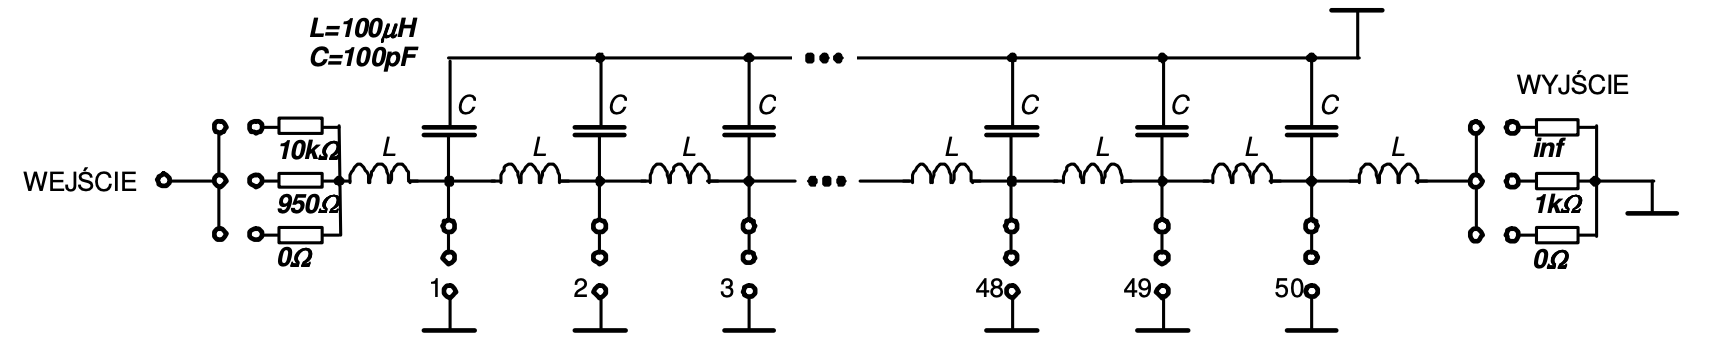
\includegraphics[width=18cm, height=4cm]{schemat}
\caption{Schemat modelu linii długiej}
\end{figure}

\section{Pomiary i wyniki}

\subsection{Badanie przesyłu impulsów prostokątnych  przez linię długą}

\subsubsection{$R = R_{f}$, $\rho = 0$ - linia dopasowana na wejściu i wyjściu}
\begin{figure}[h]
\centering
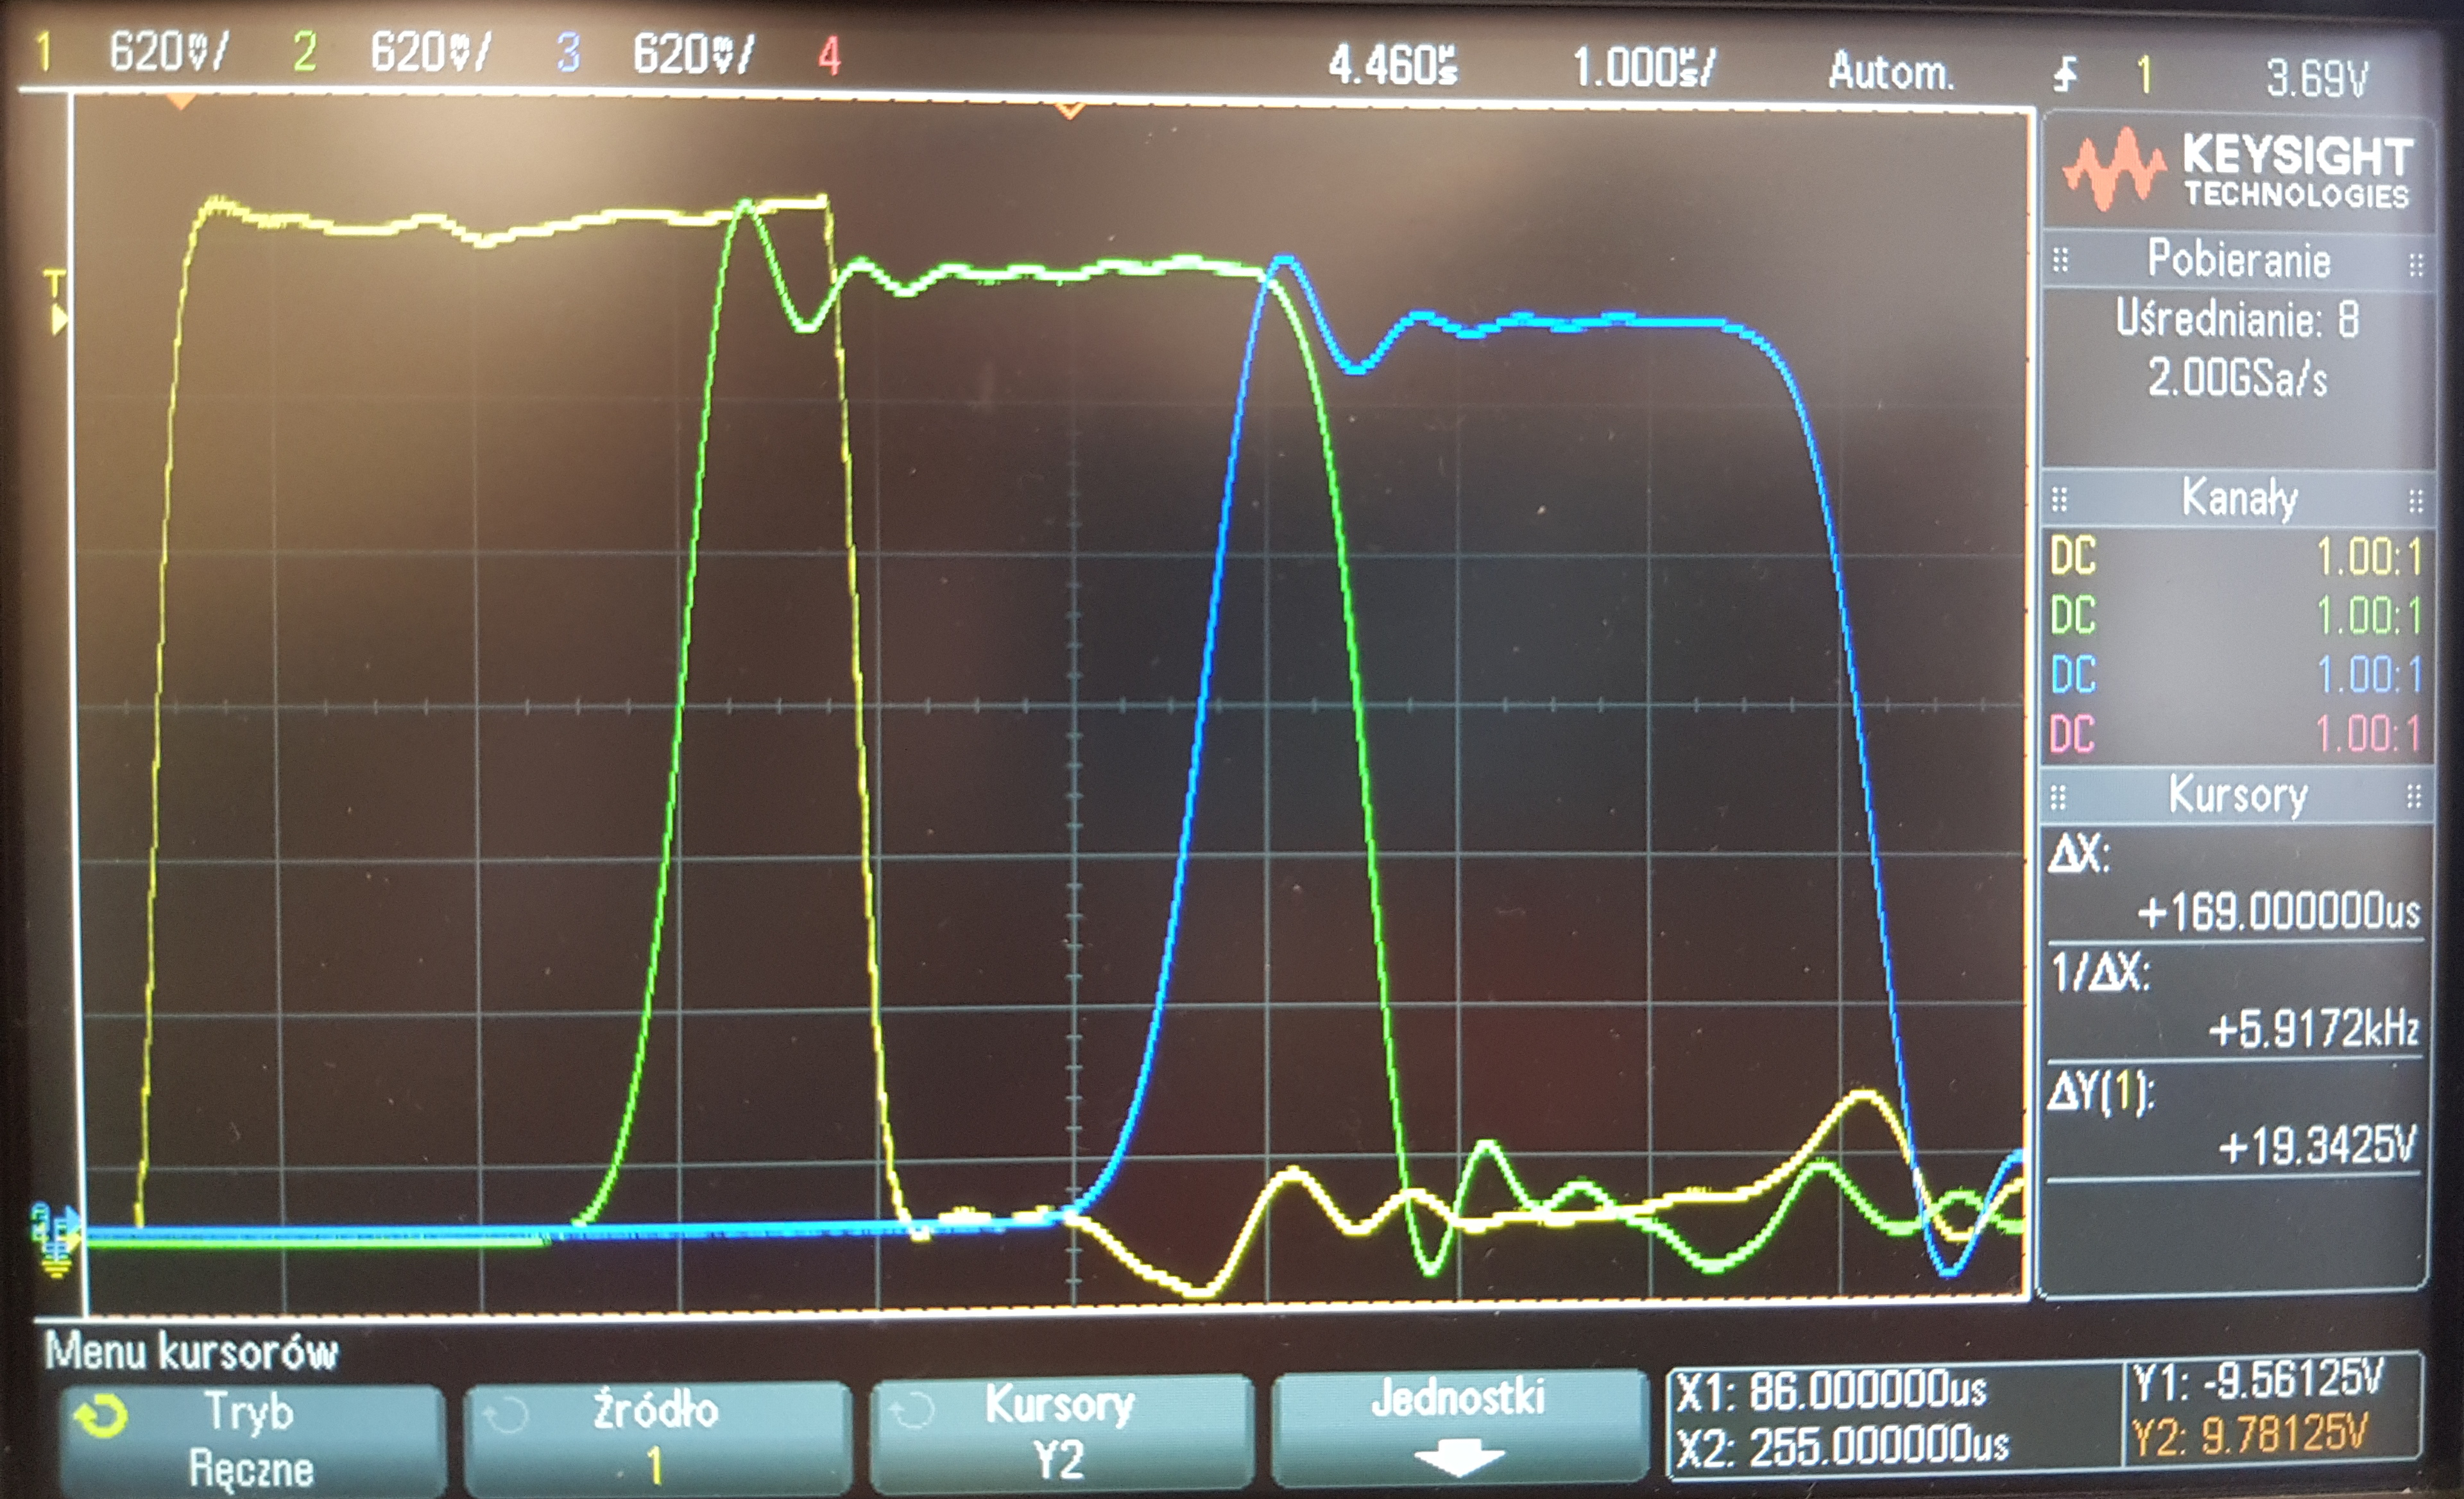
\includegraphics[width=15cm, height=9cm]{a_r=rf}
\caption{Przebieg napięcia w poszczególnych punktach linii długiej}
\begin{tabular}{cl}
\crule[yellow]{1cm}{0.4cm}  & Wejście \\
\crule[green]{1cm}{0.4cm}   & $\frac{L}{2}$  \\
\crule[blue]{1cm}{0.4cm}      & Wyjście \\
\end{tabular}
\end{figure}

Czas opóźnienia linii: \\
\begin{itemize}
\item W punkcie $\frac{L}{2}$: $t_{0} = 2.6 \mu s$
\item Na wyjściu: $t_{0} = 5.12 \mu s$
\end{itemize}

Czas opóźnienia linii na wyjściu możemy wyznaczyć w następujący sposób:
\begin{equation}
t_{0} = n * \sqrt{L * C} = 50 * \sqrt{100 \mu H * \SI{100}{\pico F}} = \SI{5}{\micro s} 
\end{equation}

Natomiast czas opóźnienia linii w punkcie $\frac{L}{2}$ możemy wyliczyć ze wzoru:
\begin{equation}
t_{0}(\frac{L}{2}) = \frac{n}{2} * \sqrt{L * C} = 25 * \sqrt{100 \mu H * \SI{100}{\pico F}} = \SI{2.5}{\micro s} 
\end{equation}

\begin{center}
\begin{tabular}{ @{}|c|c|c|@{} }
\hline
Punkt linii & Wartość teoretyczna [$\SI{}{\micro s}$] & Wartość zmierzona [$\SI{}{\micro s}$] \\
\hline
$\frac{L}{2}$ & 2.5 & 2.6 \\
\hline
$L$ & 5 & 5.12 \\
\hline
\end{tabular}
\end{center}

Na podstawie danych zawartych w tabeli możemy powiedzieć, iż wartość teoretyczna jest zbliżona do wartości zmierzonej przy wzięciu pod uwagę niepewności pomiarowej.

Jednocześnie jesteśmy w stanie zaobserwować spadki amplitud w kolejnych pomiarach, co spowodowane jest występowaniem oporu w linii, który zaniedbujemy w obliczeniach. 

\newpage

\subsubsection{$R = 0$, $\rho = -1$ - linia dopasowana na wejściu i zwarta na końcu}
\begin{figure}[h]
\centering
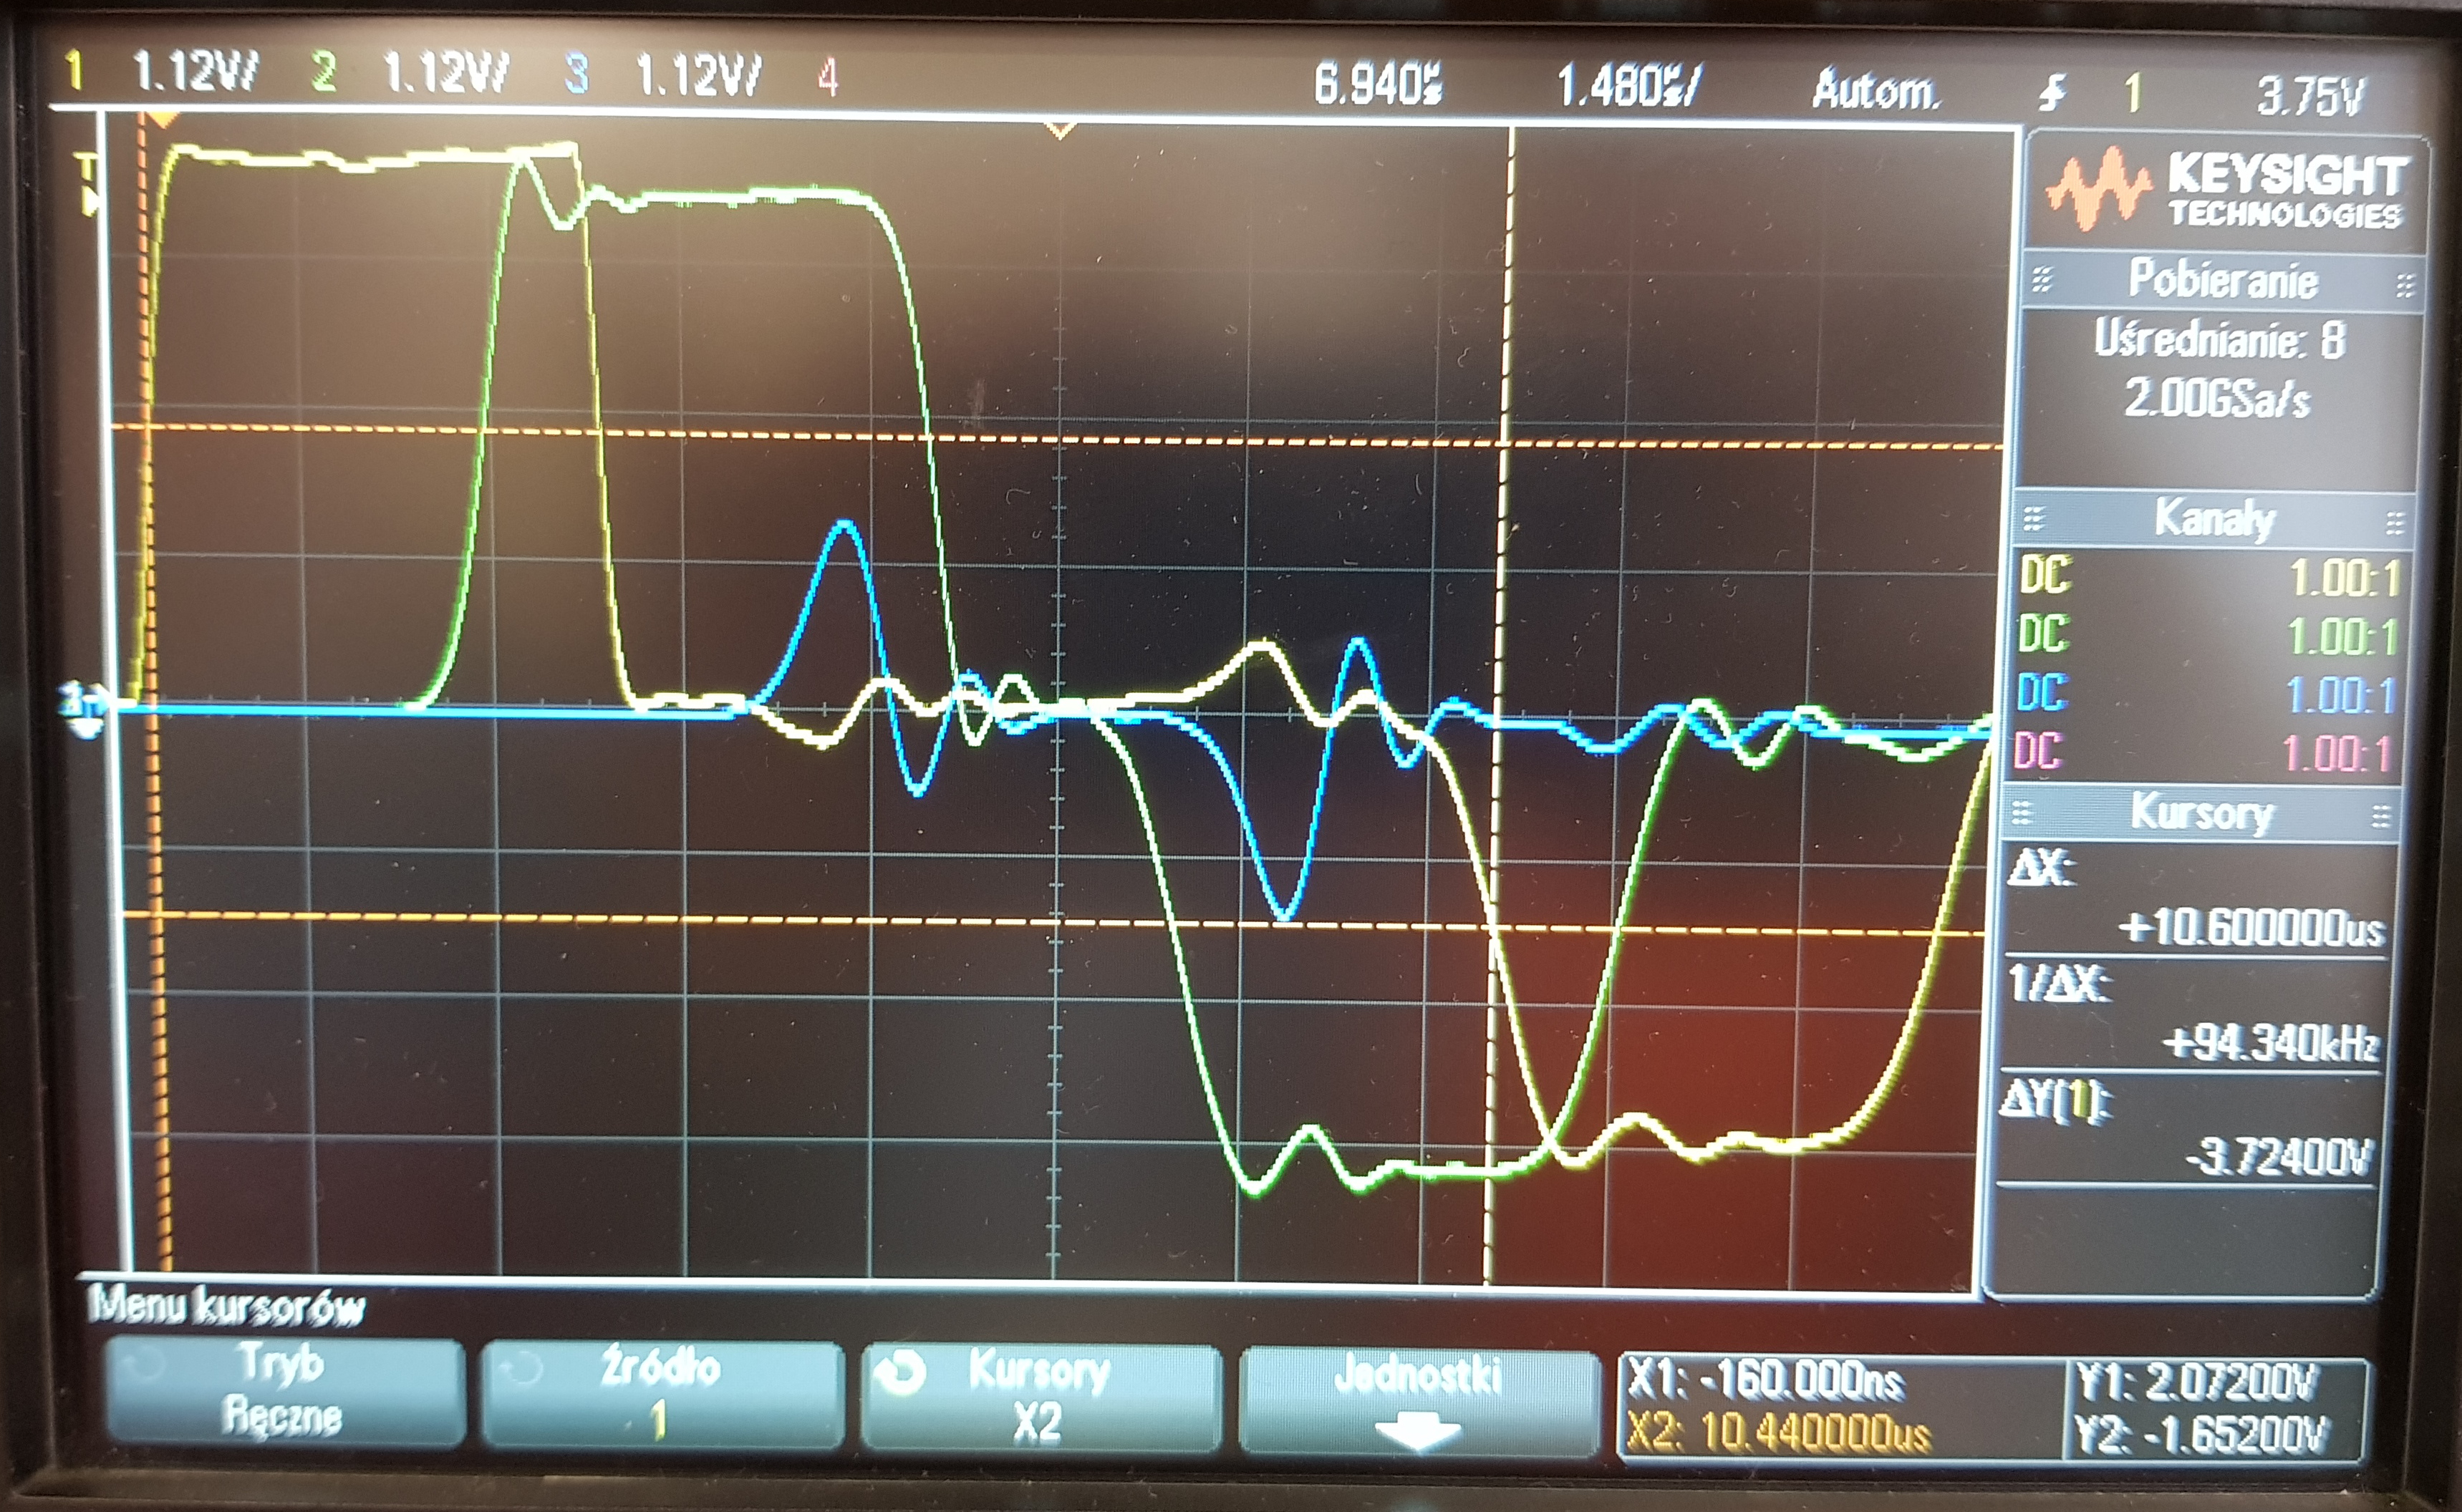
\includegraphics[width=15cm, height=9cm]{b_r=0}
\caption{Przebieg napięcia w poszczególnych punktach linii długiej}
\begin{tabular}{cl}
\crule[yellow]{1cm}{0.4cm}  & Wejście \\
\crule[green]{1cm}{0.4cm}   & $\frac{L}{2}$  \\
\crule[blue]{1cm}{0.4cm}      & Wyjście \\
\end{tabular}
\end{figure}

Czas opóźnienia linii: \\
\begin{itemize}
\item Na wejściu: $t_{0} = \SI{0}{\micro s}$, sygnał odbity pojawia się w chwili: $t = \SI{10.44}{\micro s}$
\item W punkcie $\frac{L}{2}$: $t_{0} = \SI{2.42}{\micro s} $, sygnał odbity pojawia się w chwili: $t = \SI{7,9}{\micro s}$
\item Na wyjściu: $t_{0} = \SI{5.16}{\micro s}$
\end{itemize}

Czas opóźnienia linii teoretyczny: \\
\begin{itemize}
\item Na wejściu: $t_{0} = \SI{0}{\micro s}$, sygnał odbity pojawia się w chwili: $t = \SI{10}{\micro s}$
\item W punkcie $\frac{L}{2}$: $t_{0} = \SI{2.5}{\micro s} $, sygnał odbity pojawia się w chwili: $t = \SI{7.5}{\micro s}$
\item Na wyjściu: $t_{0} = \SI{5}{\micro s}$
\end{itemize}

Amplitudy linii: \\
\begin{itemize}
\item Na wejściu: $U = \SI{4.14}{V}$, sygnał odbity: $U = \SI{-3.62}{V}$
\item W punkcie $\frac{L}{2}$: $U = \SI{4.08}{V} $, sygnał odbity $U = \SI{-3.72}{V}$
\item Na wyjściu: $U = \SI{1.4}{V}$
\end{itemize}

\paragraph{Sygnał na wyjściu powinien być równy 0V, aczkolwiek na naszym zdjęciu taki nie jest. Wynika to z faktu, iż dokonywaliśmy pomiaru nie na faktycznym końcu linii długiej, więc obserwujemy moment wygaszania sygnału w tym segmencie. \\ \, \\
Z pomiaru amplitud wynika, iż faktycznie amplituda sygnału odbitego jest przeciwna do sygnału wejściowego, ale lekko tłumiona z powodu nieidelanych własności linii, co potwierdza wartość współczynnika odbicia. \\ \, \\
Z powodu tłumienia obserwujemy coraz mniejsze amplitudy wraz z przemieszczaniem się wzdłuż linii.}

\newpage

\subsubsection{$R = \infty$, $\rho = 1$ - linia dopasowana na wejściu i rozwarta na końcu}
\begin{figure}[h]
\centering
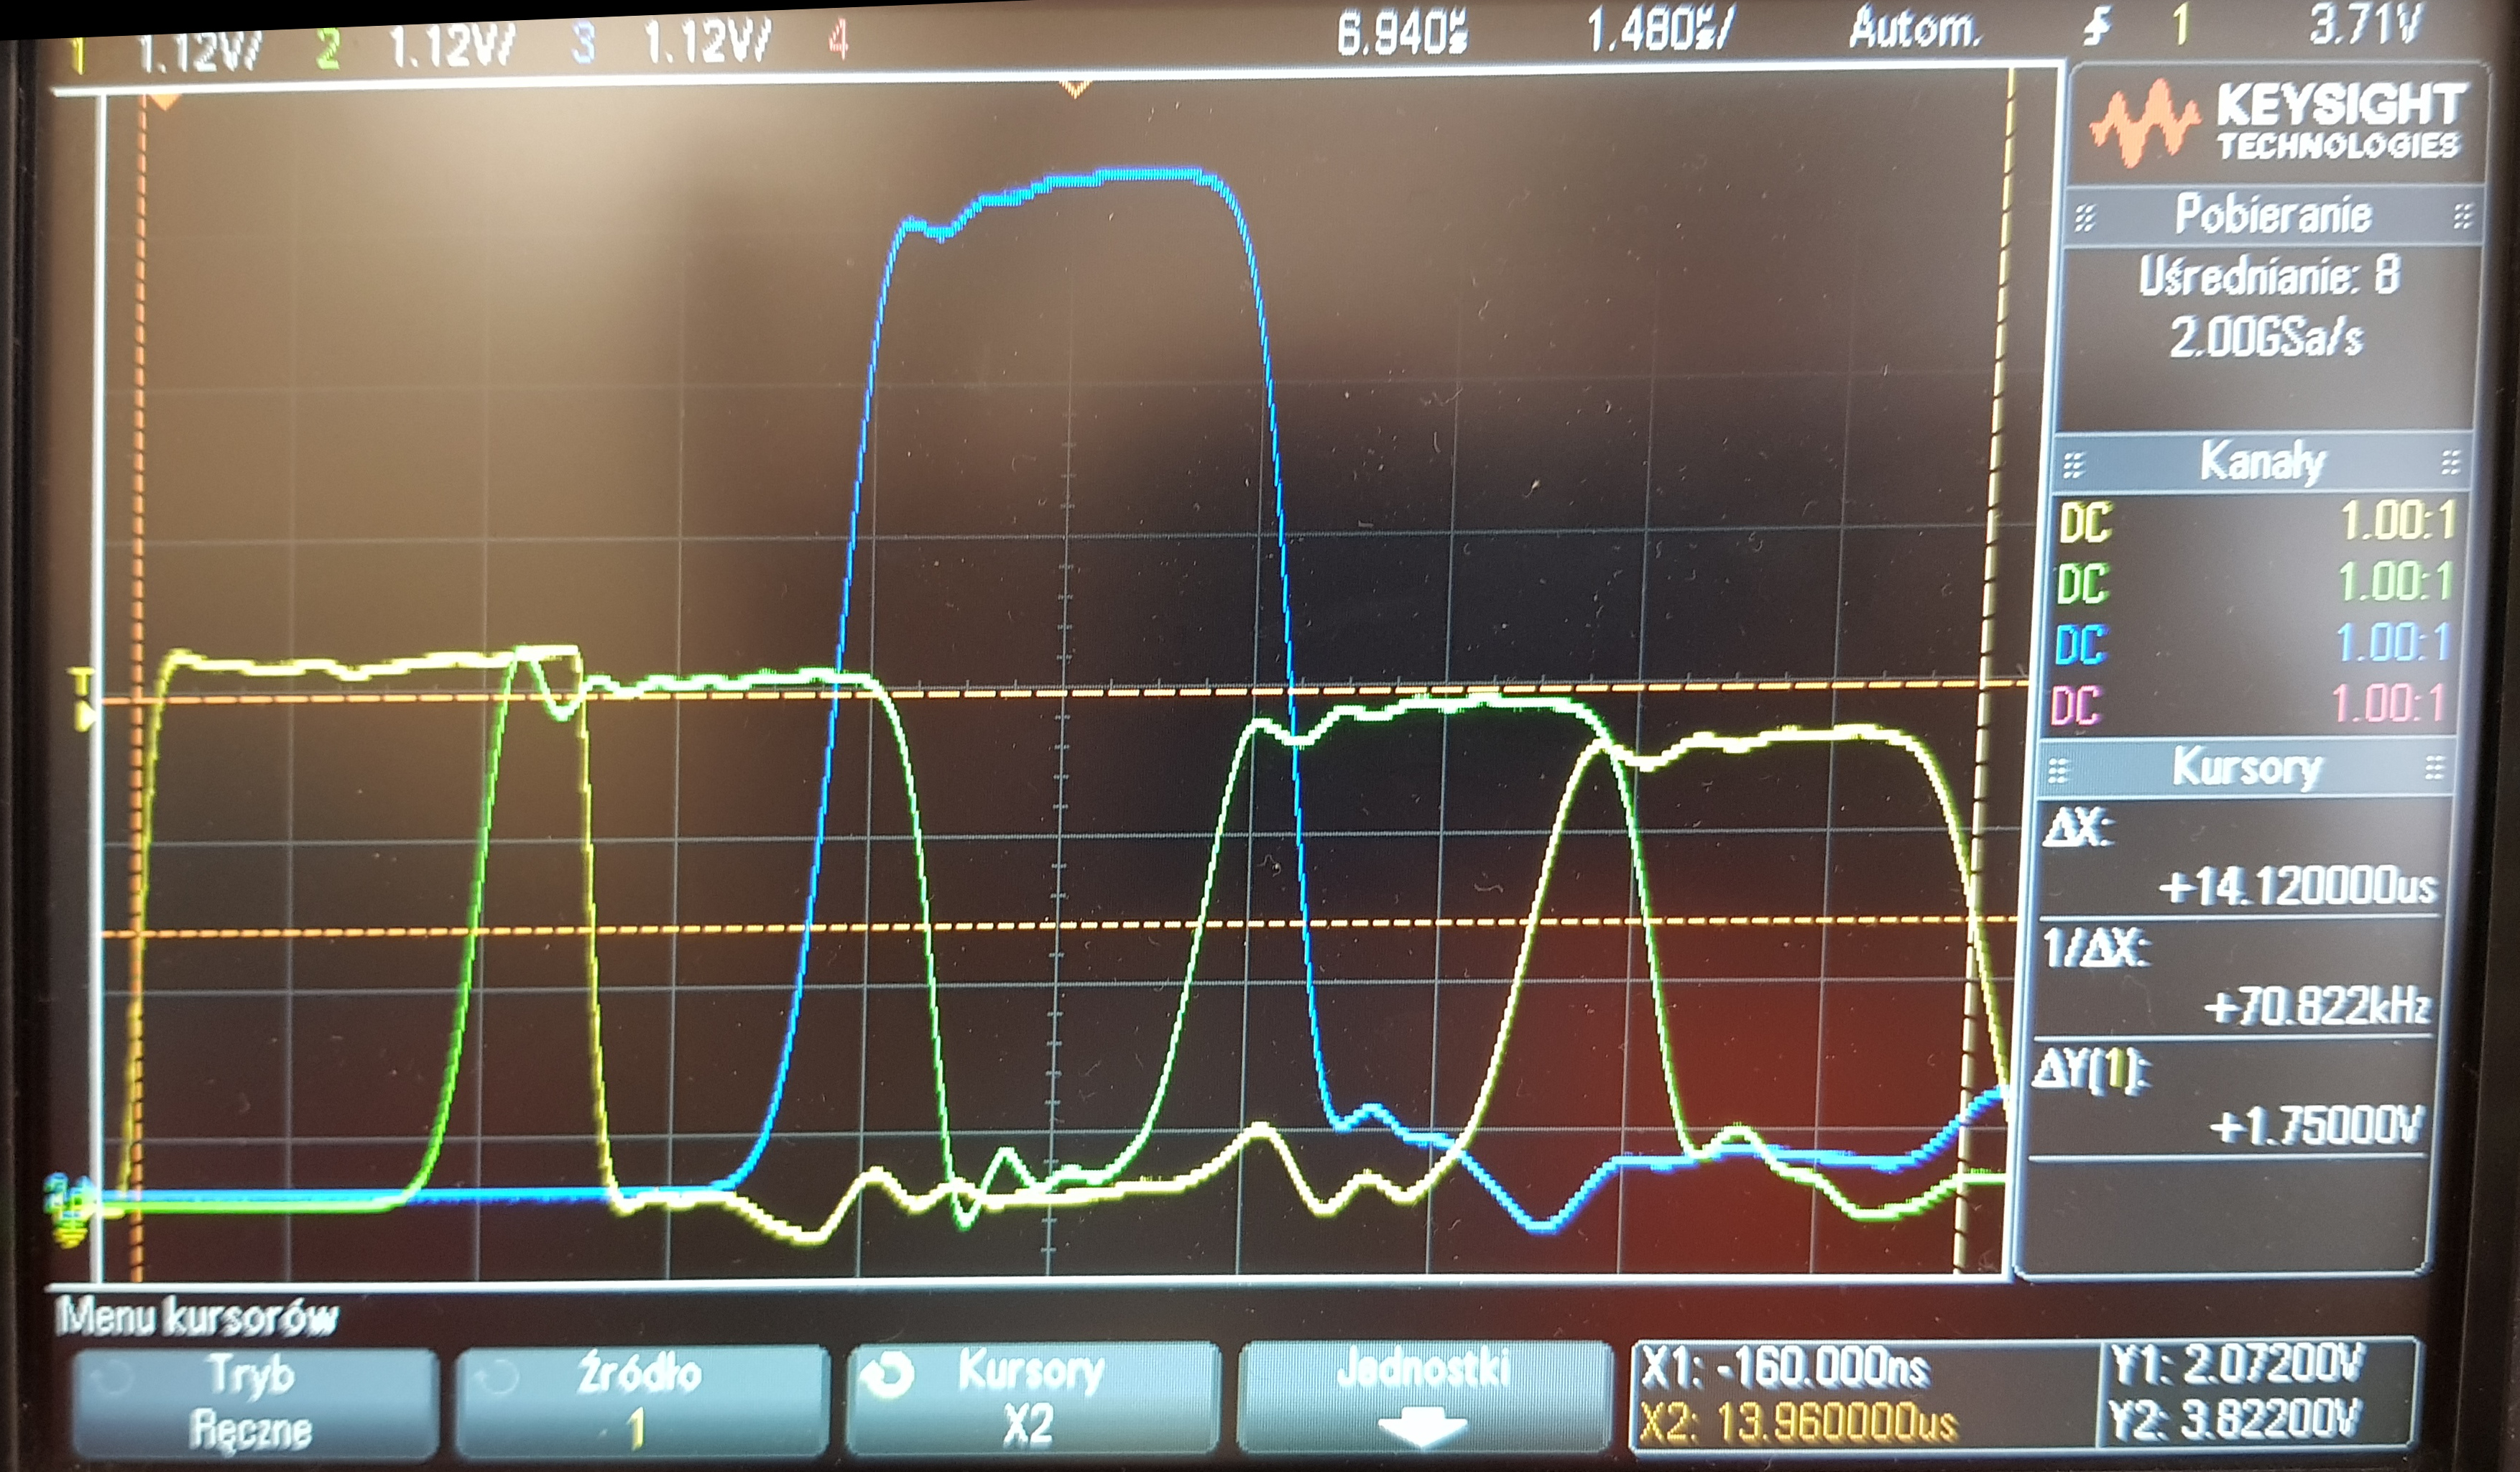
\includegraphics[width=15cm, height=9cm]{c_r=inf}
\caption{Przebieg napięcia w poszczególnych punktach linii długiej}
\begin{tabular}{cl}
\crule[yellow]{1cm}{0.4cm}  & Wejście \\
\crule[green]{1cm}{0.4cm}   & $\frac{L}{2}$  \\
\crule[blue]{1cm}{0.4cm}      & Wyjście \\
\end{tabular}
\end{figure}

Czas opóźnienia linii zmierzony: \\
\begin{itemize}
\item Na wejściu: $t_{0} = \SI{0}{\micro s}$, sygnał odbity pojawia się w chwili: $t = \SI{10.64}{\micro s}$
\item W punkcie $\frac{L}{2}$: $t_{0} = \SI{2.44}{\micro s} $, sygnał odbity pojawia się w chwili: $t = \SI{8.02}{\micro s}$
\item Na wyjściu: $t_{0} = \SI{5.16}{\micro s}$
\end{itemize}

Czas opóźnienia linii teoretyczny: \\
\begin{itemize}
\item Na wejściu: $t_{0} = \SI{0}{\micro s}$, sygnał odbity pojawia się w chwili: $t = \SI{10}{\micro s}$
\item W punkcie $\frac{L}{2}$: $t_{0} = \SI{2.5}{\micro s} $, sygnał odbity pojawia się w chwili: $t = \SI{7.5}{\micro s}$
\item Na wyjściu: $t_{0} = \SI{5}{\micro s}$
\end{itemize}

Amplitudy linii: \\
\begin{itemize}
\item Na wejściu: $U = \SI{4.15}{V}$, sygnału odbitego: $U = \SI{3.48}{V}$
\item W punkcie $\frac{L}{2}$: $U = \SI{4.04}{V} $, sygnału odbitego $U = \SI{3.72}{V}$
\item Na wyjściu: $U = \SI{7.65}{V}$
\end{itemize}

\paragraph{Jak widać na powyższym rysunku sygnał na wyjściu jest superpozycją fali wejściowej i odbitej o równych amplitudach i tej samej fazie. \\ \, \\
Zgodnie z zamieszczonym wykresem, możemy zaobserwować tłumiące właściwości linii - sygnał w punkcie $\frac{L}{2}$ ma amplitudę mniejszą niż sygnał na wejściu.}

\newpage

\subsection{Badanie przesyłu impulsów prostokątnych o czasie trwania dłuższym niż czas opóźnienia  przez linię długą}

\paragraph{Czas trwania impulsu dla naszej grupy został wyznaczony przez prowadzącego wynosi: $\SI{22}{\micro s}$.}

\subsubsection{$R = 0$, $\rho = -1$ - linia dopasowana na wejściu i zwarta na końcu}
\begin{figure}[h]
\centering
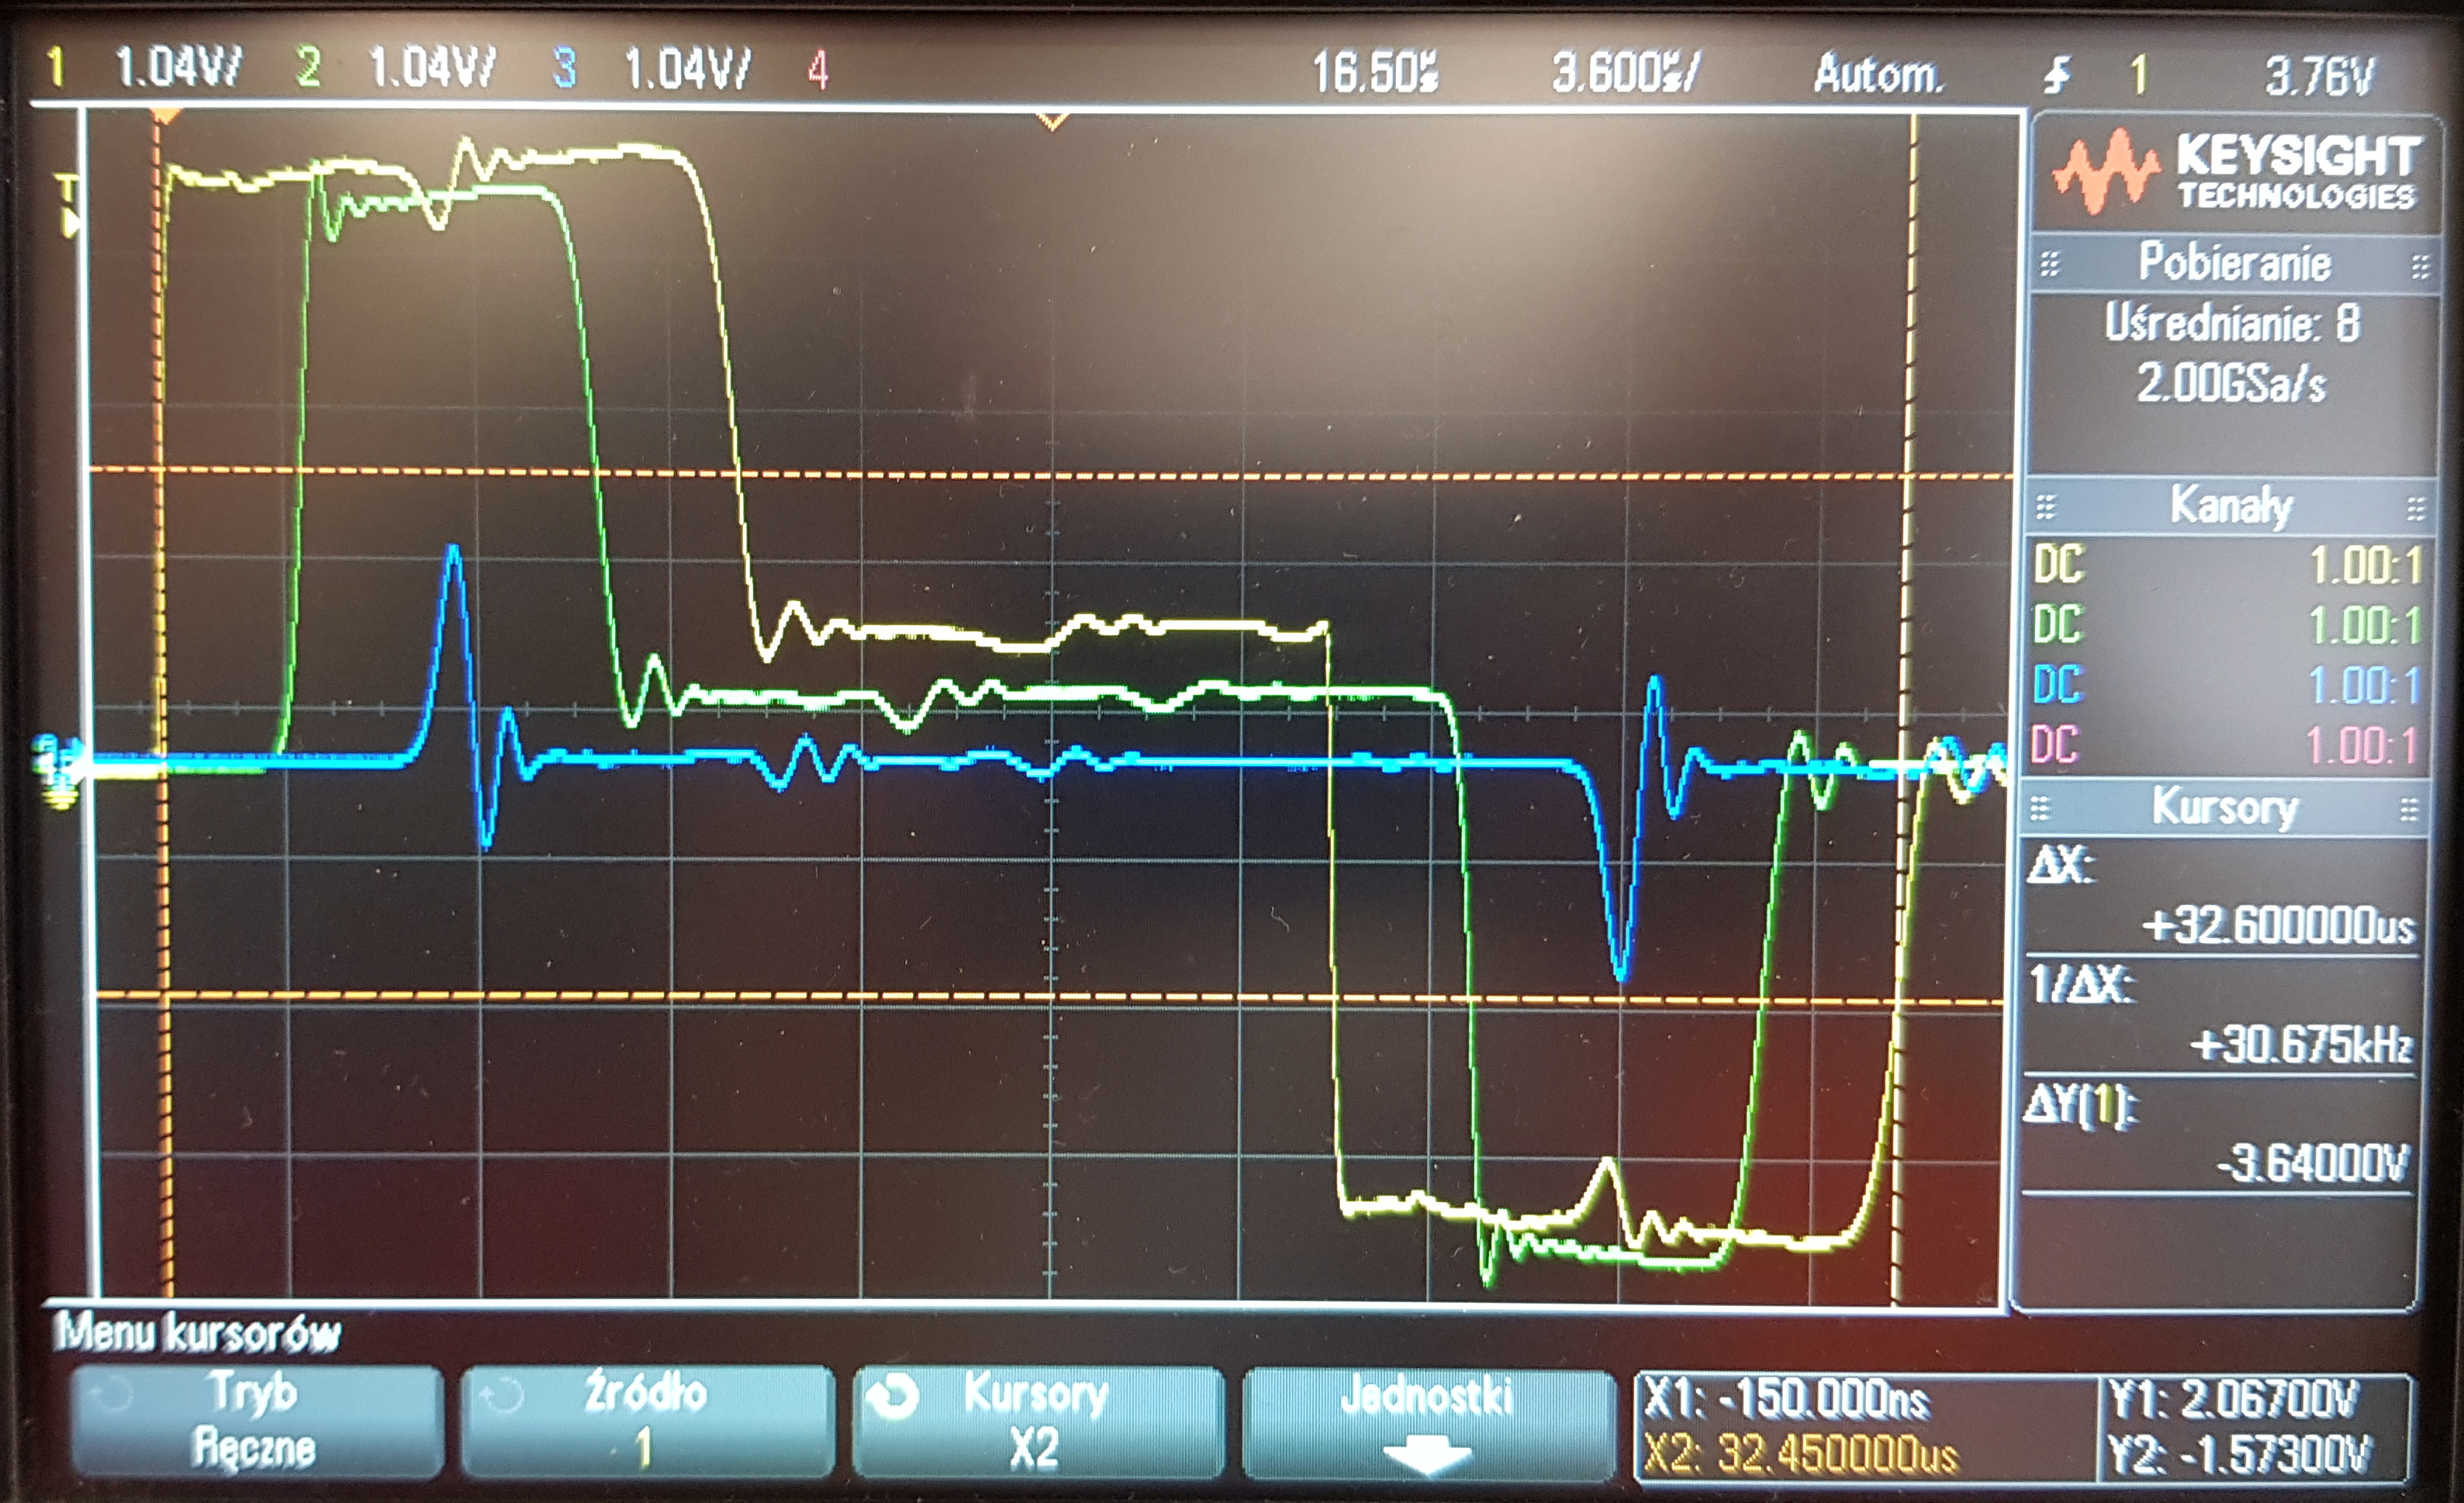
\includegraphics[width=15cm, height=9cm]{2_a_r=0}
\caption{Przebieg napięcia w poszczególnych punktach linii długiej}
\begin{tabular}{cl}
\crule[yellow]{1cm}{0.4cm}  & Wejście \\
\crule[green]{1cm}{0.4cm}   & $\frac{L}{2}$  \\
\crule[blue]{1cm}{0.4cm}      & Wyjście \\
\end{tabular}
\end{figure}

Czas przebiegu sygnału: \\
\begin{itemize}
\item Na wejściu: $t_{0} = \SI{0}{\micro s}$, sygnał odbity pojawia się w chwili: $t = \SI{10.7}{\micro s}$
\item W punkcie $\frac{L}{2}$: $t_{0} = \SI{2.45}{\micro s} $, sygnał odbity pojawia się w chwili: $t = \SI{24.35}{\micro s}$
\end{itemize}

Czas przebiegu sygnału teoretyczny: \\
\begin{itemize}
\item Na wejściu: $t_{0} = \SI{0}{\micro s}$, sygnał odbity pojawia się w chwili: $t = \SI{10}{\micro s}$
\item W punkcie $\frac{L}{2}$: $t_{0} = \SI{2.5}{\micro s} $, sygnał odbity pojawia się w chwili: $t = \SI{25}{\micro s}$
\end{itemize}

Amplitudy linii: \\
\begin{itemize}
\item Na wejściu: $U = \SI{4.15}{V}$, sygnału odbitego: $U = \SI{-3.14}{V}$
\item W punkcie $\frac{L}{2}$: $U = \SI{3.95}{V} $, sygnału odbitego $U = \SI{-3.35}{V}$
\end{itemize}

\paragraph{W tym przypadku również obserwujemy wygaszanie fali na wyjściu linii długiej, jednak nie jest ono całkowite z powodu niedokładności modelu linii długiej oraz z powodu punktu pomiarowego, który nie znajdował się dokładnie w końcu linii. \\ \, \\
Natomiast różne poziomy zer wynikają z tego, iż sygnał nadawany nakłada się z sygnałem odbitym, a nie są sobie równe z powodu efektu tłumienia. }

\newpage

\subsubsection{$R = \infty$, $\rho = 1$ - linia dopasowana na wejściu i rozwarta na końcu}
\begin{figure}[h]
\centering
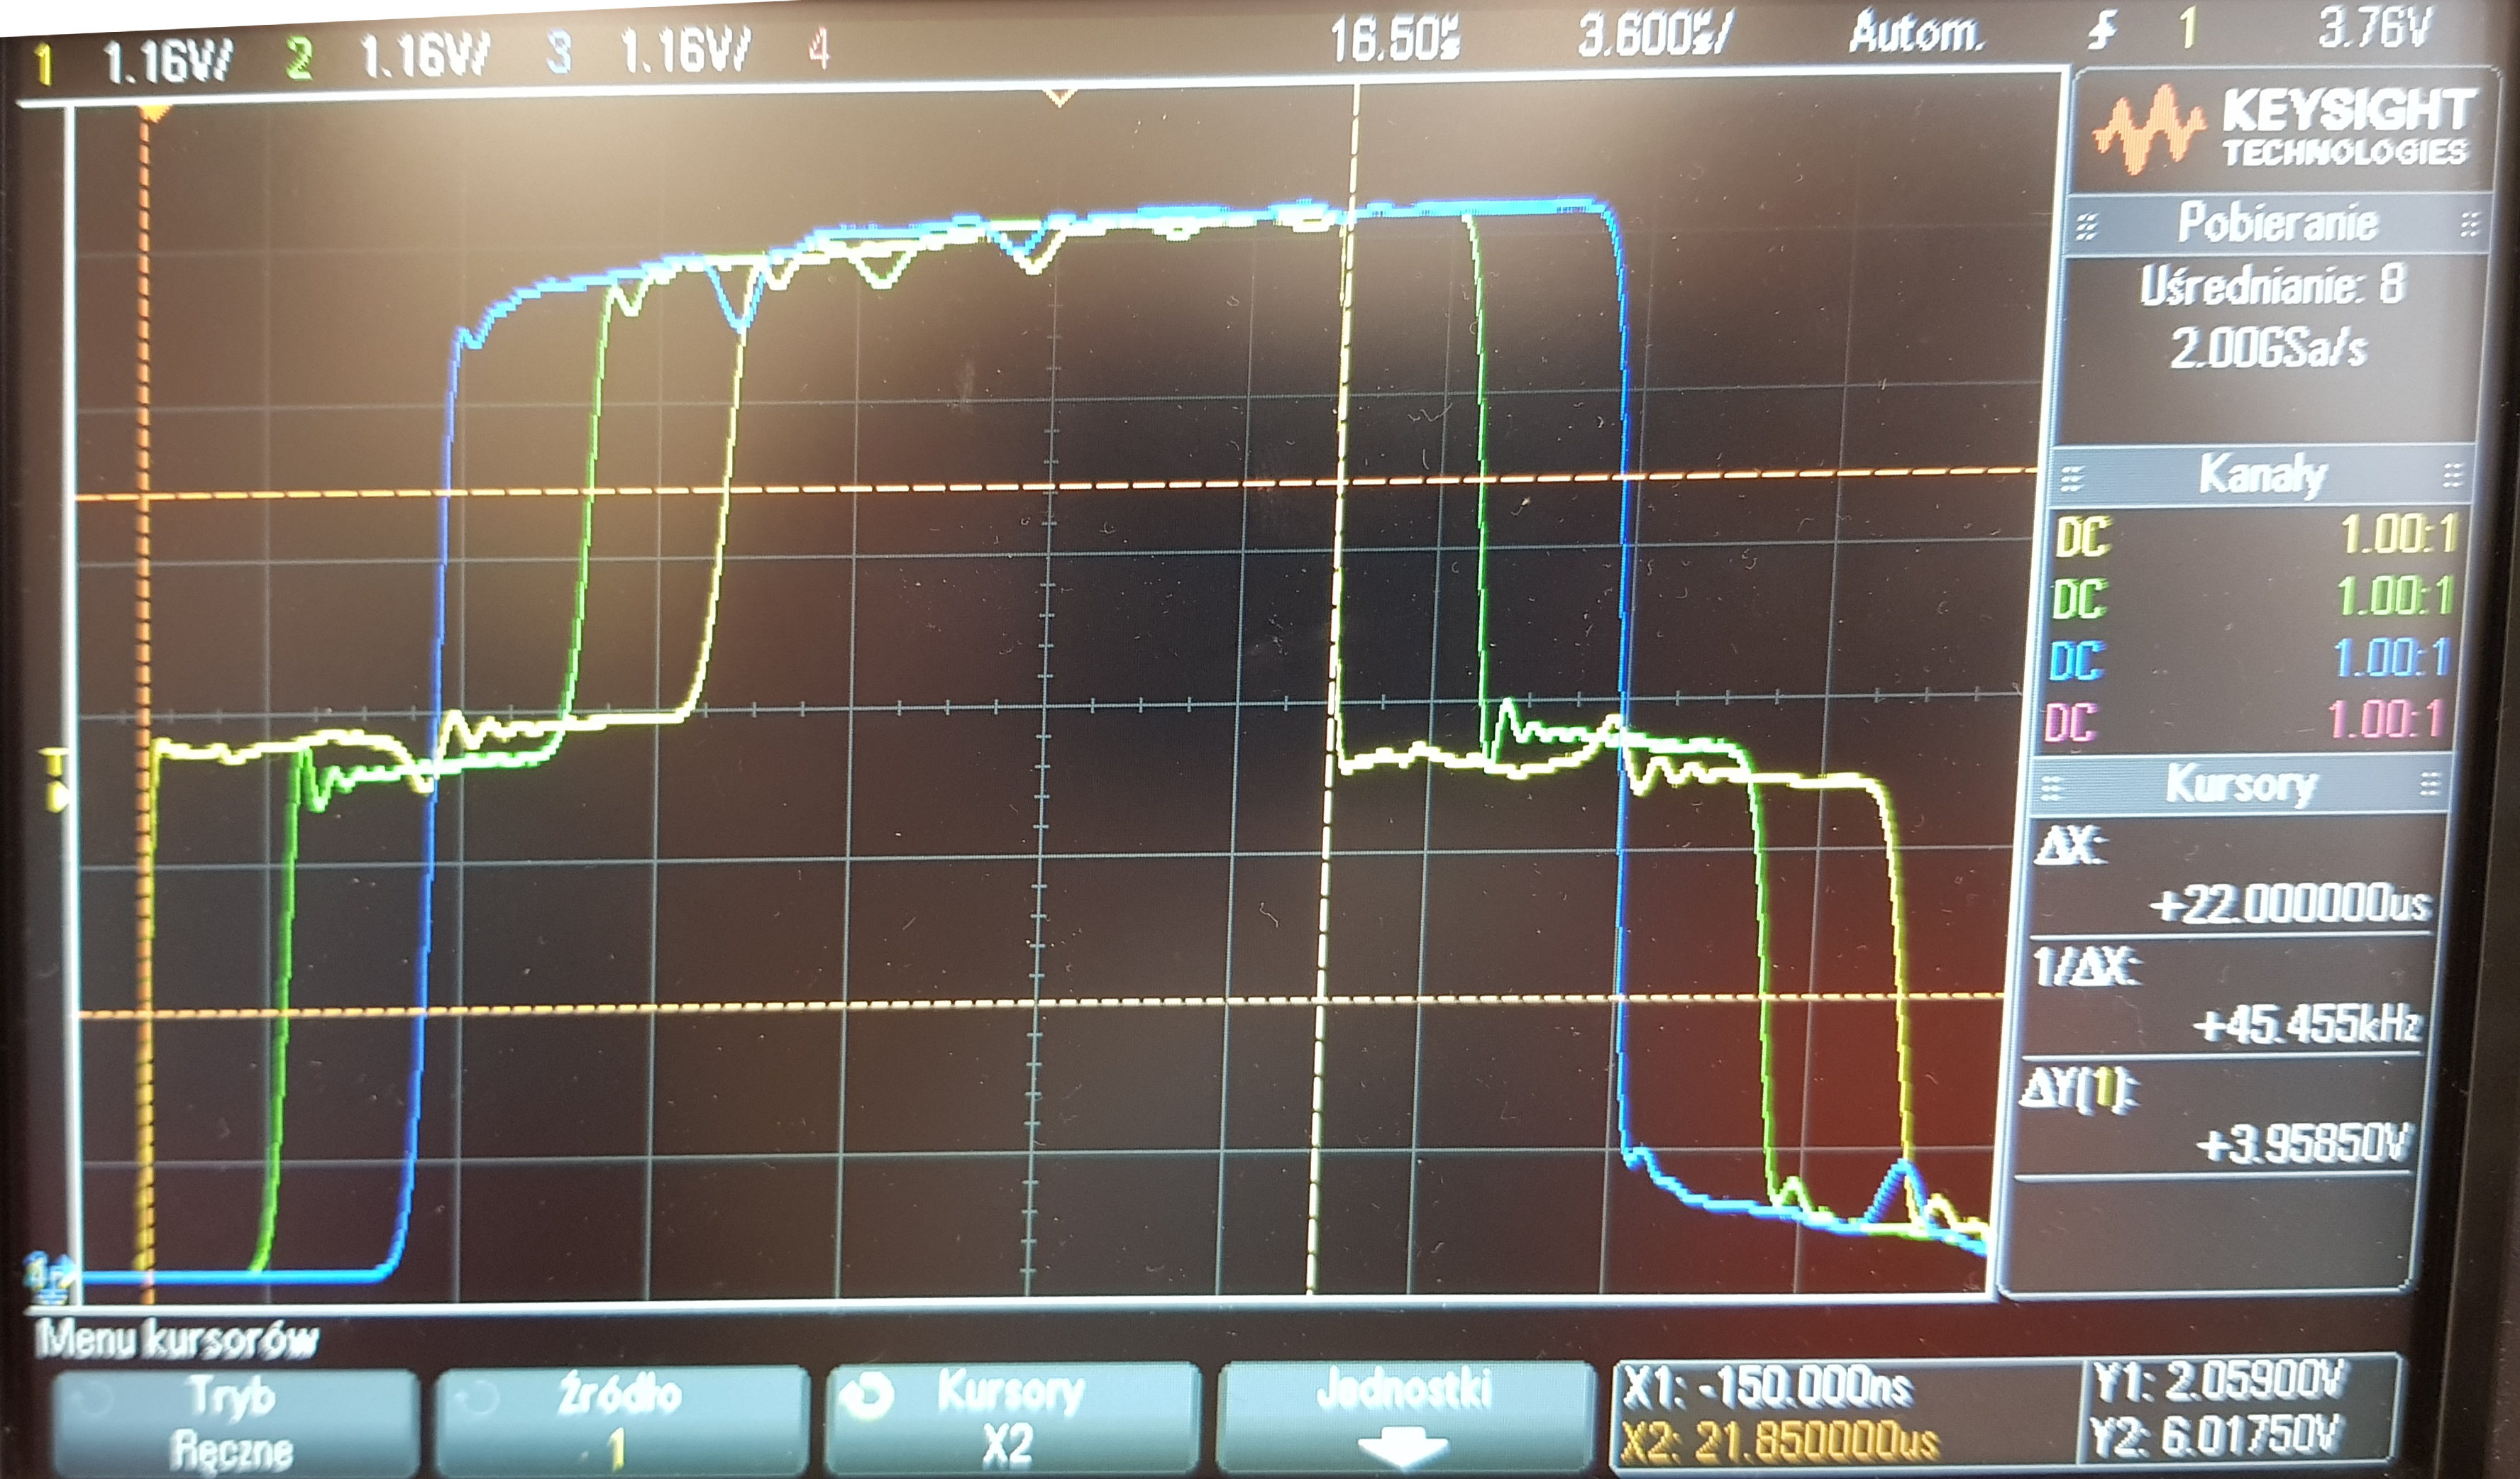
\includegraphics[width=15cm, height=9cm]{2_b_r=inf}
\caption{Przebieg napięcia w poszczególnych punktach linii długiej}
\begin{tabular}{cl}
\crule[yellow]{1cm}{0.4cm}  & Wejście \\
\crule[green]{1cm}{0.4cm}   & $\frac{L}{2}$  \\
\crule[blue]{1cm}{0.4cm}      & Wyjście \\
\end{tabular}
\end{figure}

Czas przebiegu sygnału: \\
\begin{itemize}
\item Na wejściu: $t_{0} = \SI{0}{\micro s}$, sygnał odbity pojawia się w chwili: $t = \SI{10.65}{\micro s}$
\item W punkcie $\frac{L}{2}$: $t_{0} = \SI{2.4}{\micro s} $, sygnał odbity pojawia się w chwili: $t = \SI{8.15}{\micro s}$
\item Na wyjściu: $t_{0} = \SI{4.95}{\micro s}$
\end{itemize}

Czas przebiegu sygnału teoretyczny: \\
\begin{itemize}
\item Na wejściu: $t_{0} = \SI{0}{\micro s}$, sygnał odbity pojawia się w chwili: $t = \SI{10}{\micro s}$
\item W punkcie $\frac{L}{2}$: $t_{0} = \SI{2.5}{\micro s} $, sygnał odbity pojawia się w chwili: $t = \SI{7.5}{\micro s}$
\end{itemize}

Amplitudy linii: \\
\begin{itemize}
\item Na wejściu: $U = \SI{4.11}{V}$, sygnału odbitego: $U = \SI{7.91}{V}$
\item W punkcie $\frac{L}{2}$: $U = \SI{3.97}{V} $, sygnału odbitego $U = \SI{8.04}{V}$
\item Na wyjściu: $U = \SI{7.93}{V}$
\end{itemize}

\paragraph{Jak widać po powyższych danych amplituda jest superpozycją amplitudy wejściowej oraz odbitej na wyjściu, co jest zgodne z współczynnikiem odbicia, powodując jej zwiększenie o 2 razy. \\ \, \\
Amplitudy w kolejnych punktach pomiarowych są coraz niższe, co jest spowodowane niedokładnością modelu linii, którym dysponowaliśmy. }

\newpage

\subsection{Obserwacja efektu pojemnościowego linii}

\begin{figure}[h]
\centering
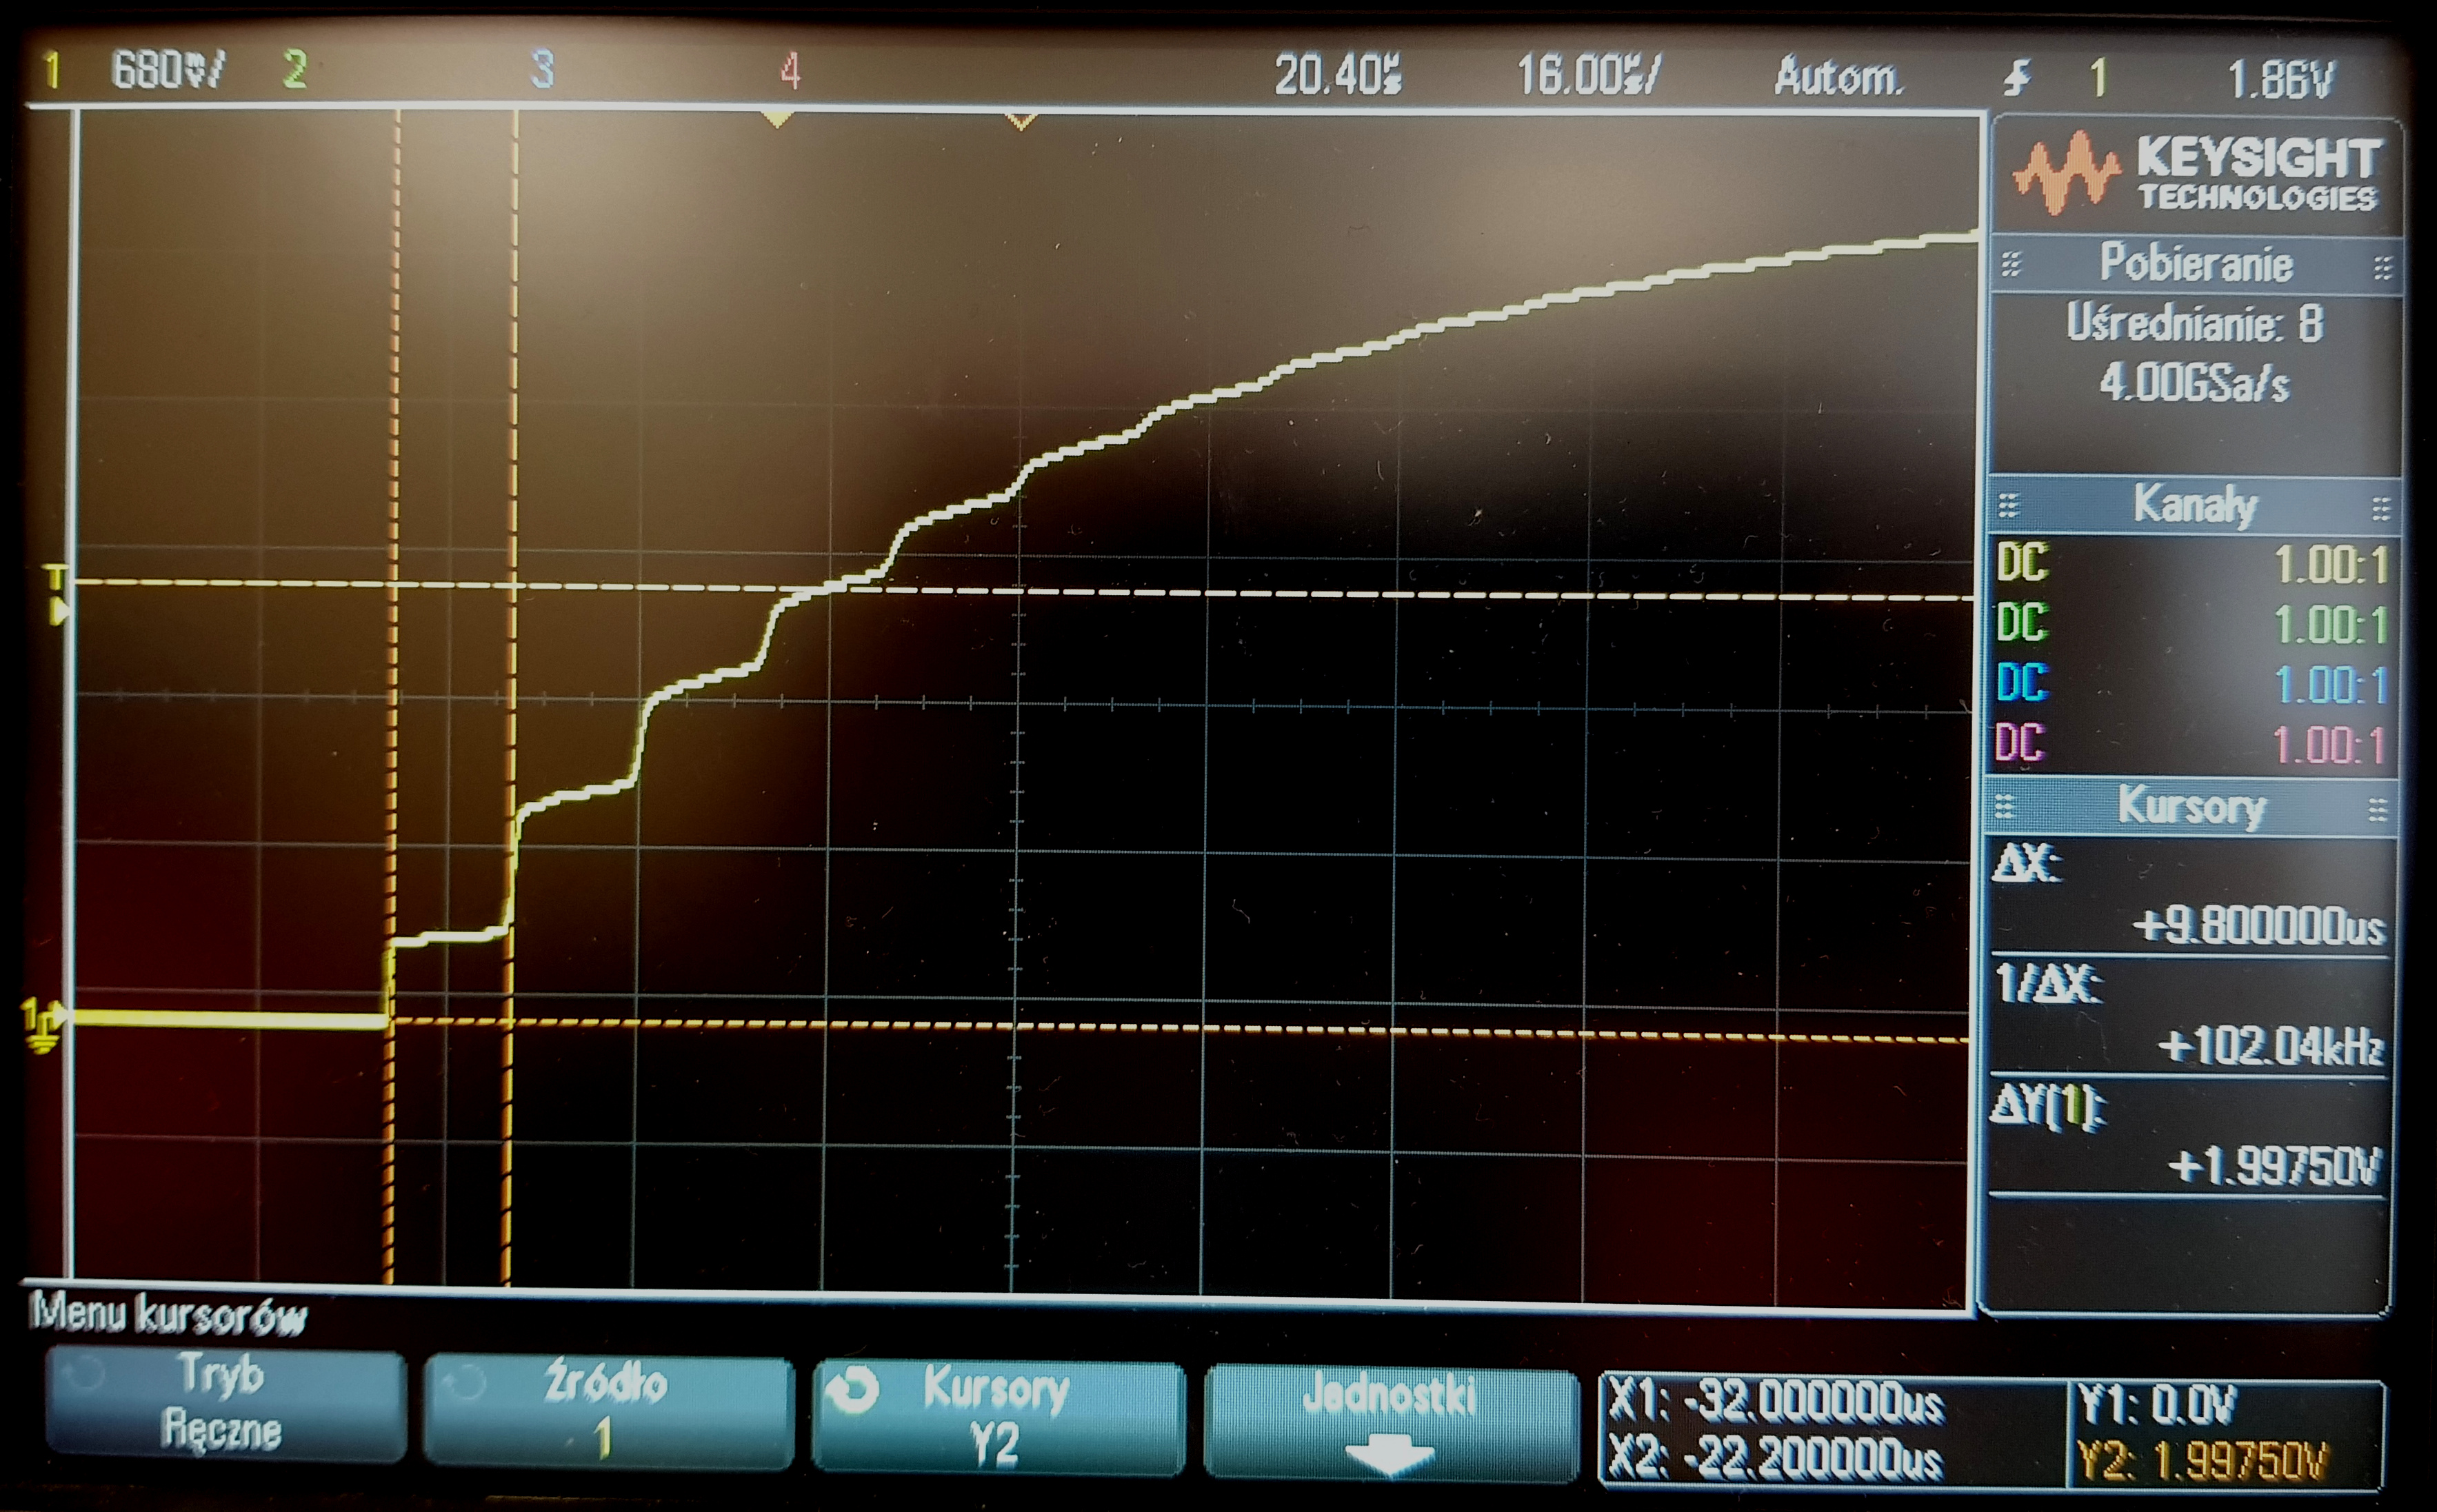
\includegraphics[width=15cm, height=9cm]{2_c}
\caption{Efekt pojemnościowy obserwowany za pomocą przebiegu napięcia}
\end{figure}

\paragraph{Wymuszenie wejściowe $U_{in} = 3V$}
\paragraph{Współczynnik odbicia: $\rho = \frac{\frac{R}{R_{f}} -1}{\frac{R}{R_{f}} +1} = \frac{9}{11}$}

\paragraph{Teoretyczna długość każdego schodka wynosi $t = 2 * t_{0}$, co wynika z przejścia sygnału od końca linii i jego powrót.}

\newpage

\begin{table}[h!]
\begin{center}
\begin{scriptsize}
\begin{tabular}{|l|l|l|}
\hline
Nr. schodka & Amplituda $U$ [mV] & Czas rozpoczęcia $t$ [$\mu s$] \\
\hline
1 & 382 & 0 \\
2 & 1030 & 9.8 \\
3 & 1560 & 20.4 \\
4 & 2380 & 31.4 \\
5 & 2660 & 42 \\
6 & 2890 & 52.2 \\
\hline
\end{tabular}
\caption{Tabela zawierająca informację o kolejnych "schodkach" spowodowanych efektem pojemnościowym}
\label{table:1}
\end{scriptsize}
\end{center}
\end{table}

\begin{figure}[h]
\centering
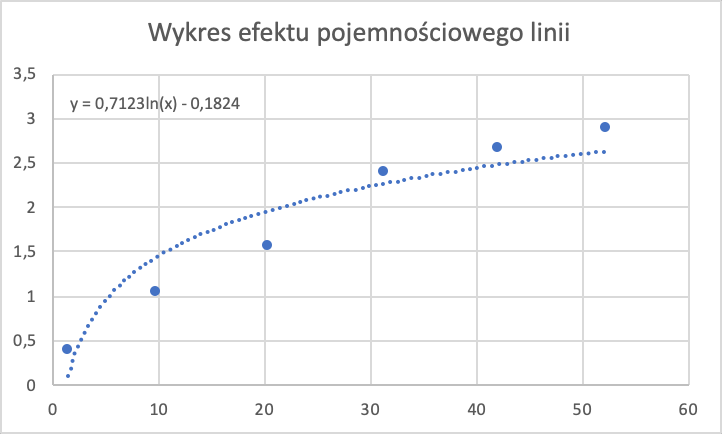
\includegraphics[width=10cm, height=6cm]{2_c_wykr}
\caption{Wykres pomiarów efektu pojemnościowego oraz jego interpolacja logarytmiczna}
\end{figure}



\newpage

\subsection{Obserwacja efektów spowodowanych nieidealnymi własnościami rzeczywistego modelu }

\begin{figure}[h]
\centering
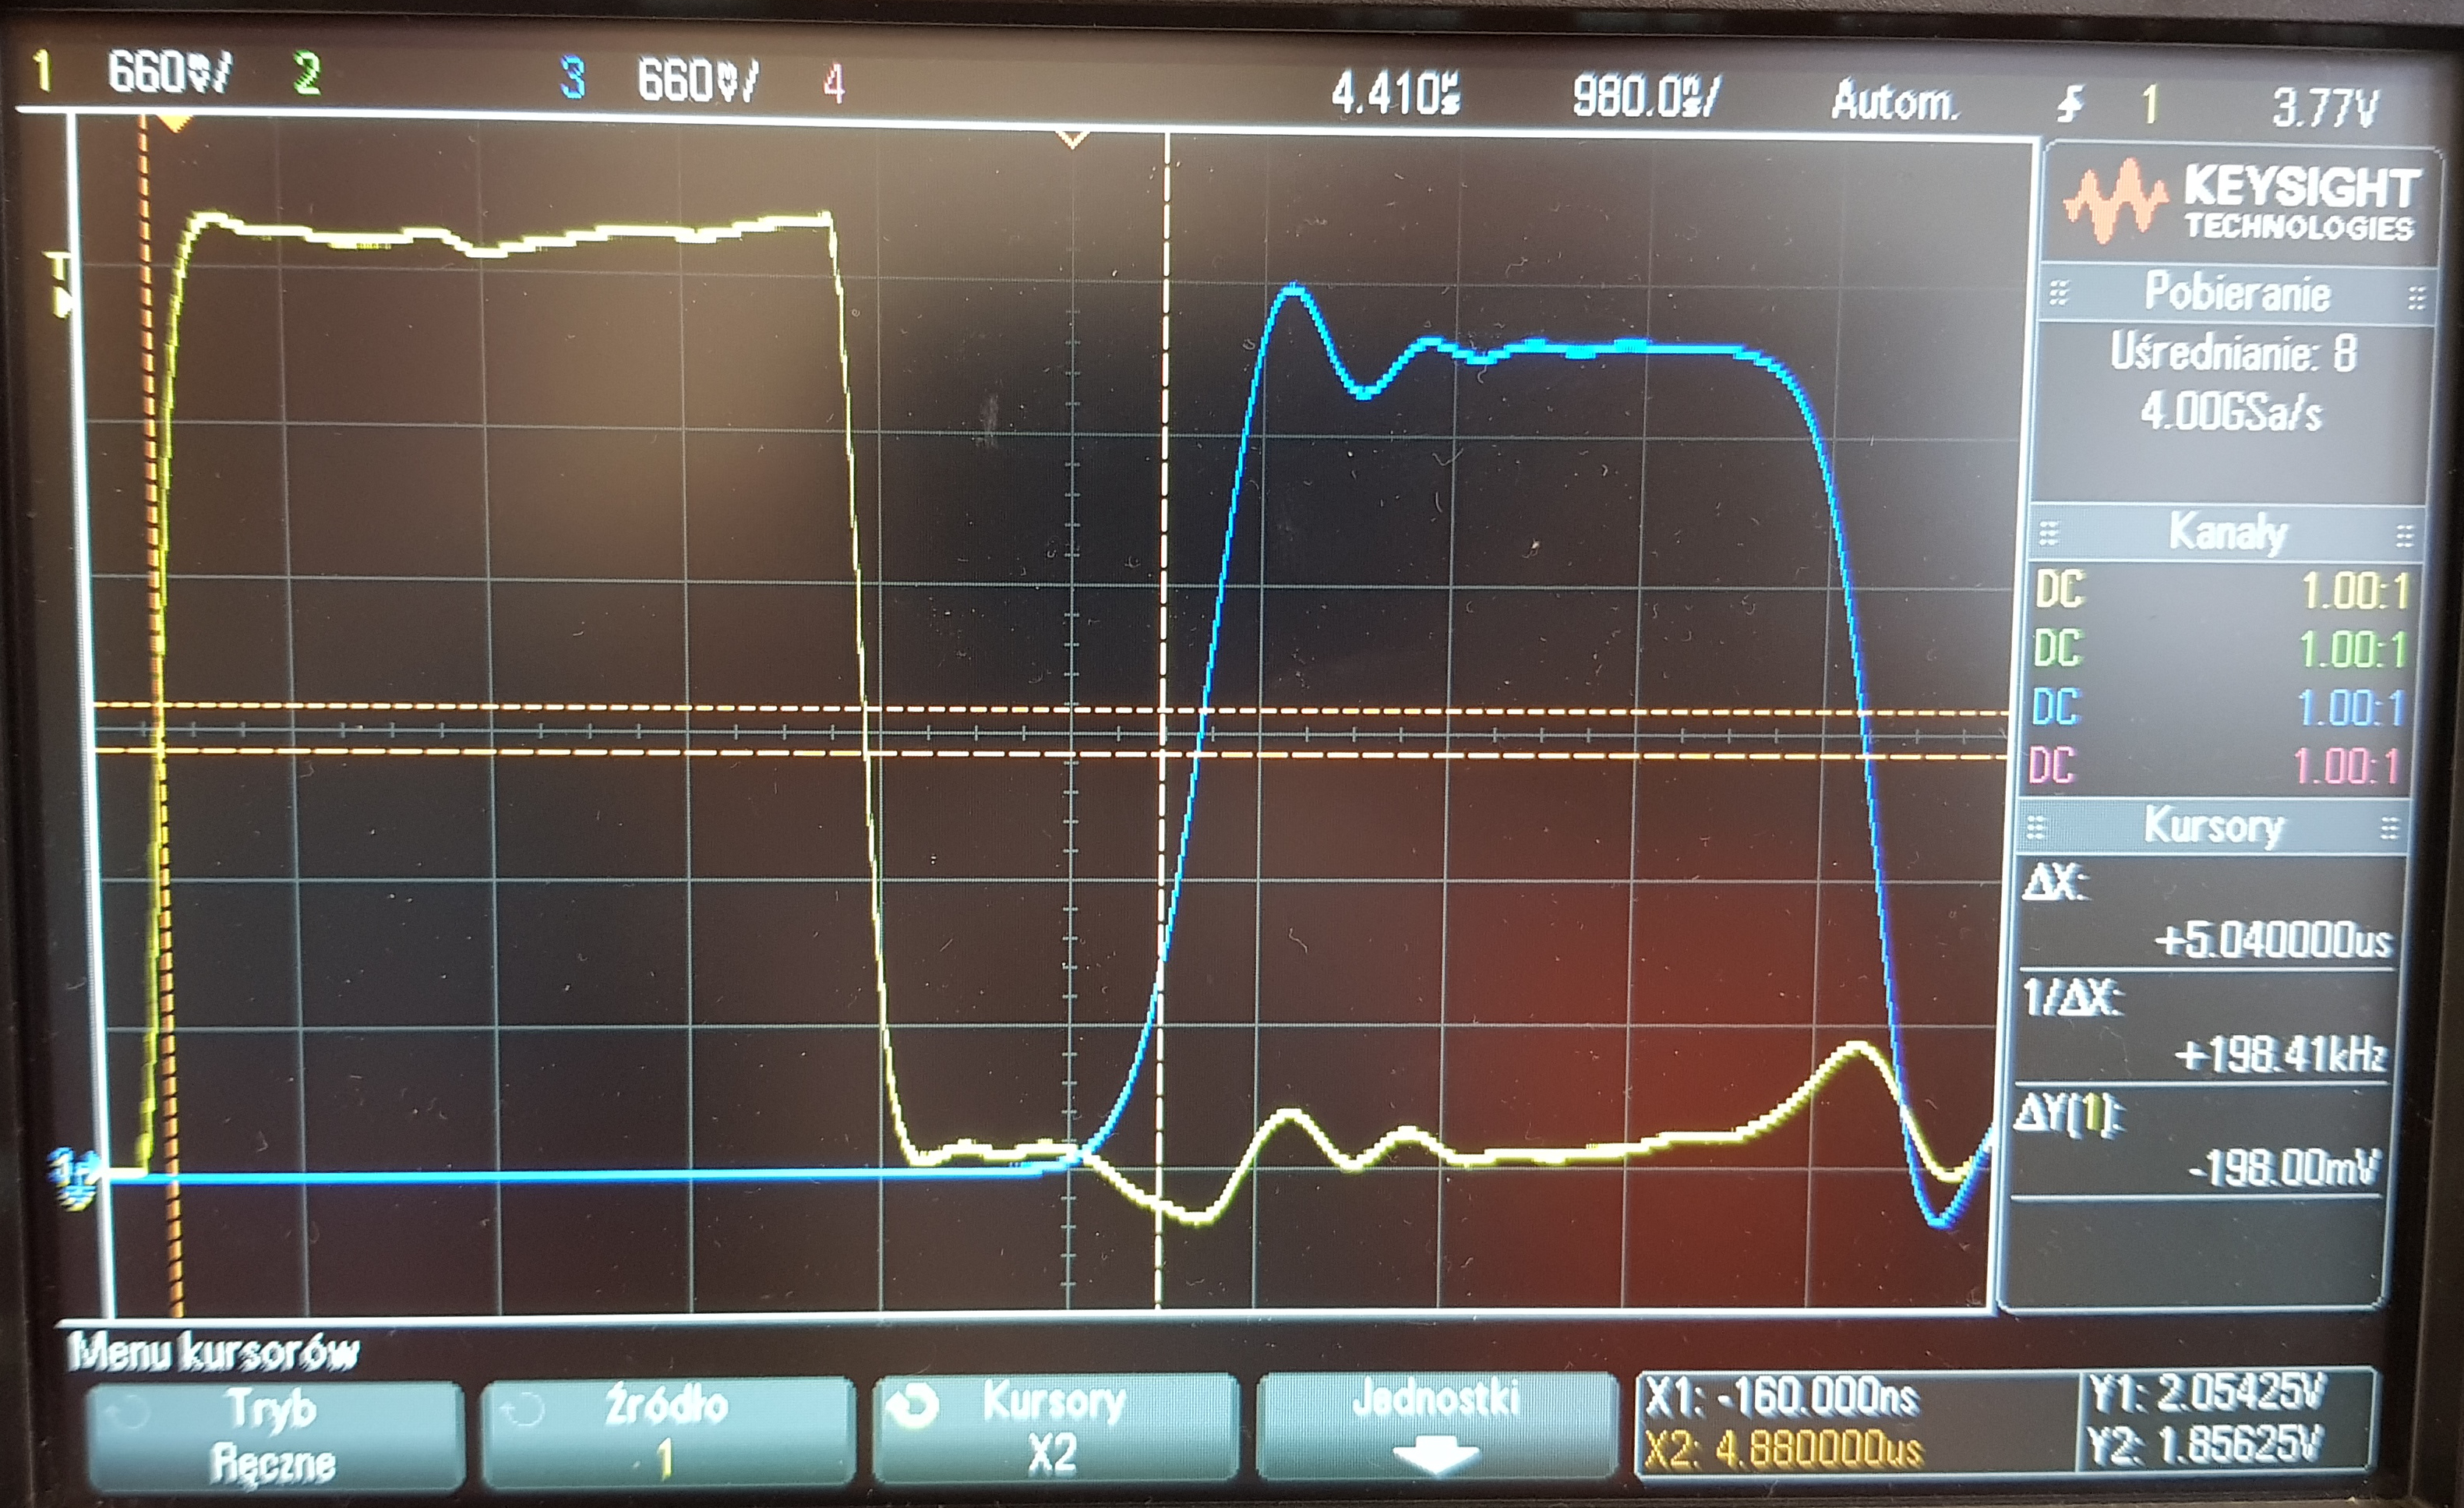
\includegraphics[width=15cm, height=9cm]{3}
\caption{Przebieg napięcia w poszczególnych punktach linii długiej}
\crule[yellow]{1cm}{0.4cm} - Wejście \\
\crule[blue]{1cm}{0.4cm} - Wyjście \\
\end{figure}

Z powodu realnego niezerowego oporu możemy zaobserwować efekt tłumienia. Poniżej wypisane są istotne wartości dla tego zjawiska:
\begin{center}
$A_{in} = 4.09V$ \\
$A_{out} = 3.7V$ \\
$tr_{in} = 217ns$ \\
$tr_{out} = 586ns$ \\
$tr_{w} = \sqrt{tr_{out}^2 - tr_{in}^2} = 585.97ns$ \\
$t_{0} = \SI{5.26}{\micro s}$ \\
$k = 0.904$ \\
$k_{dB} = \SI{-0.870}{dB}$ \\
$F_{g} = 5.97Hz$ \\
Teoretyczne: \\
$tr_{w} = 128ns$ \\
$F_{g} = 2.79Hz$ \\
\end{center}

\newpage

\subsection{Badanie transmisji krótkiego impulsu prostokątnego przez kabel koncentryczny}

\begin{figure}[h]
\centering
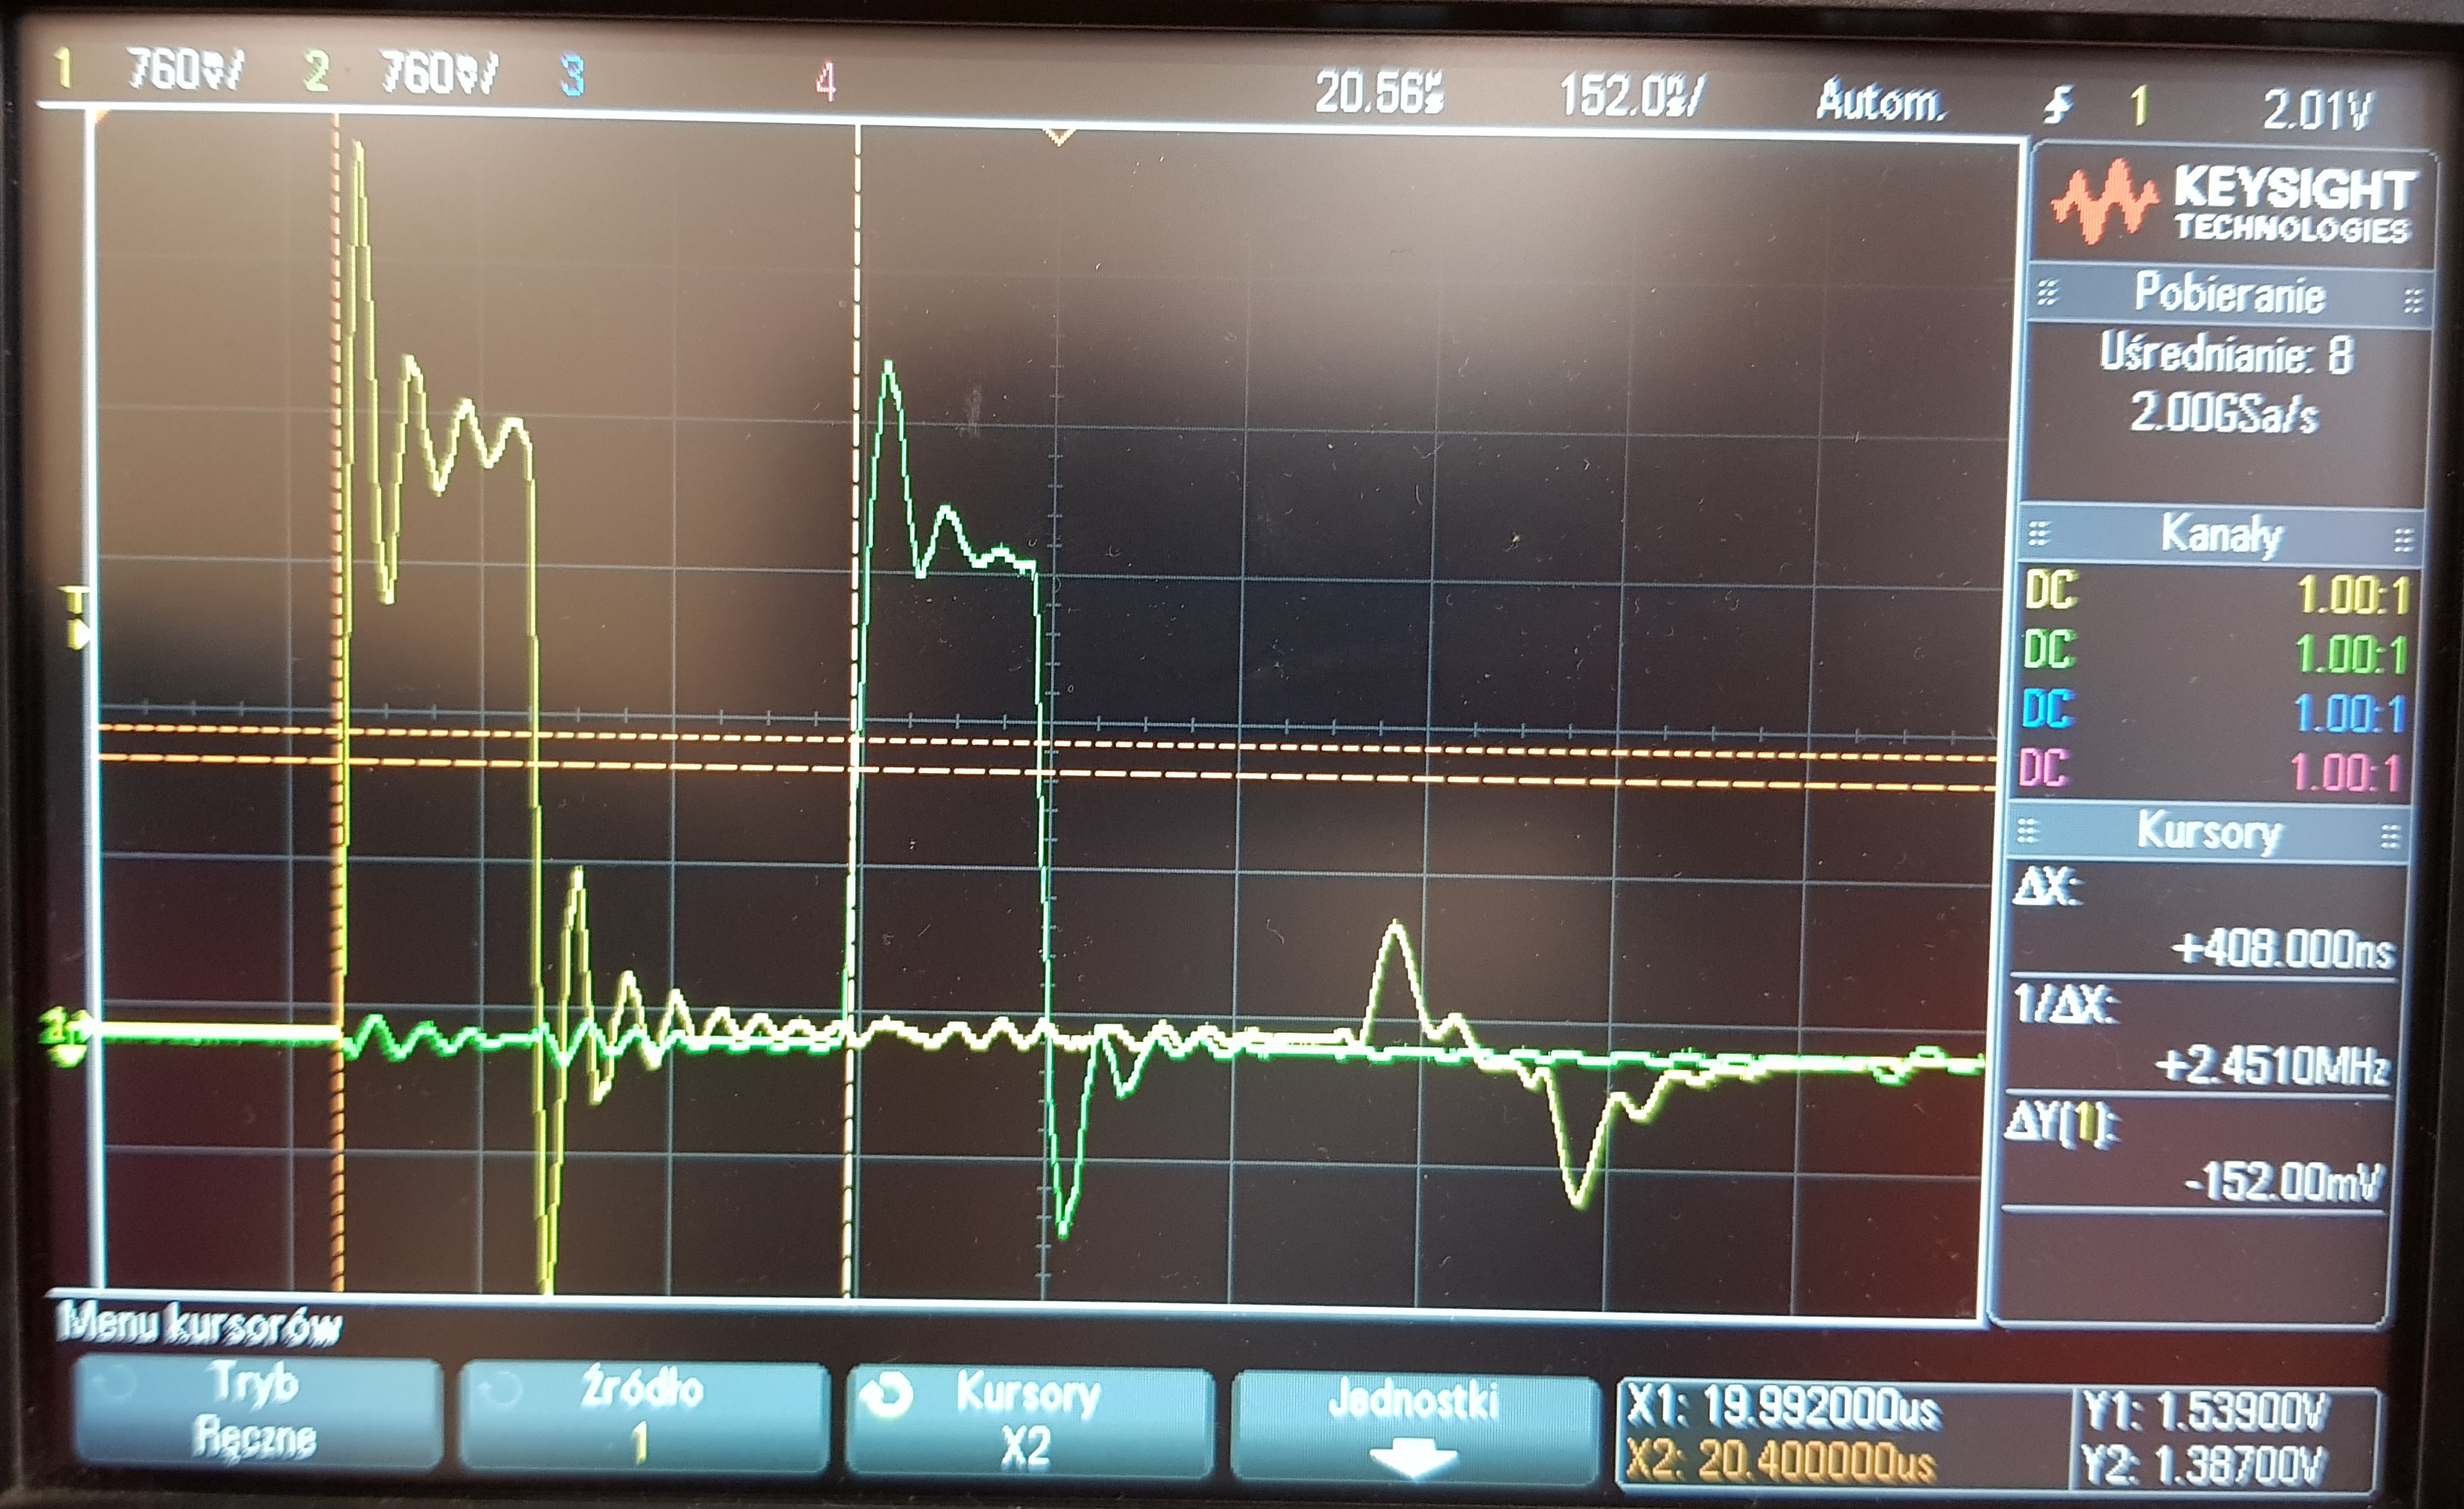
\includegraphics[width=15cm, height=9cm]{4}
\caption{Przebieg napięcia}
\crule[yellow]{1cm}{0.4cm} - Wejście \\
\crule[green]{1cm}{0.4cm} - Wyjście \\
\end{figure}

\paragraph{W naszym przypadku zamiast znanej długości kabla, znaliśmy czas opóźnienia na jednostkę długości kabla koncentrycznego $t_{l} = 5 \frac{ns}{m}$. Dokonując zmian na rezystorze wyjściowym sprawdzaliśmy, czy występuje odbicie. W momencie, gdy go nie zaobserwowaliśmy byliśmy w stanie wyznaczyć wartość rezystancji falowej, które jest równa rezystancji na naszym oporniku wejściowym. Ponadto wyznaczyliśmy poniższe wartości: }

\begin{itemize}
\item $A_{in} = 3.07V$
\item $A_{out} = 2.72V$
\item $tr_{w} = 10.13ns$
\item Rezystancja charakterystyczna:  $r_{f} = \SI{41.52}{\Omega}$
\item Współczynnik transmisji: $k = 0.885$
\item Współczynnik transmisji [dB]: $k = \SI{-1.051}{dB}$
\item Czas opóźnienia: $t_{0} = \SI{408}{ns}$
\item Czas narastania $V_{IN}$: $tr_{IN} = \SI{6.42}{ns}$
\item Czas narastania $V_{OUT}$: $tr_{OUT} =\SI{12}{ns} $
\end{itemize}

Przy takich odczytach jesteśmy w stanie wyznaczyć doświadczalnie długość kabla koncentrycznego ze wzoru:
\begin{equation}
l = \frac{t_{0}}{t_{l}} = 81.6m
\end{equation}

\end{justify}
\end{document}